\notetoself{This chapter is taken from my transfer report. I need to
rework it to integrate it correctly within the present thesis.}


Safety has been defined as a syntactical constraint. Since Game
Semantics is by essence syntax-independent, it seems difficult at
first sight to give a game-semantic characterization of a syntactic restriction such as the Safety Condition.
In fact, the Correspondence Theorem makes such analysis possible since it allows us to regard the plays of a strategy
as sequences of nodes of some AST of the term.


The main theorem of this chapter (theorem
\ref{thm:safe_ptr_recoverable}) states that pointers in a play of
the strategy denotation of a safe term can be uniquely recovered
from O-questions' pointers and from the underlying sequence of
moves. The proof is in several steps. We start by introducing the
notion of \emph{P-incrementally-justified strategies} and prove that
for plays of such strategies, pointers emanating from P-moves can be
reconstructed uniquely from the underlying sequences of moves and
from O-moves' pointers. We then introduce the notion of
\emph{incrementally-bound computation trees} and prove that
incremental-binding coincides with P-incremental-justification
(proposition \ref{prop:Nher_incrbound_iff_incrjustified}).


Finally, we show that safe simply-typed terms in $\beta$-normal form
have incrementally\--bound computation trees, consequently their
game denotation is P-incrementally-justified.


The first section of this chapter is concerned only with the safe $\lambda$-calculus without interpreted constants. In the next
section we extend the result by taking into account the interpreted
constants of \pcf\ and \ialgol. We define the language safe \ialgol\
(resp. safe \pcf) to be the fragment of \ialgol\ (resp. \pcf) where
the application and abstraction rules are constrained the same way
as in the safe $\lambda$-calculus. We show that safe \pcf\ terms are
denoted by P-incrementally-justified strategies and we give the key
elements for a possible extension of the result to Safe Idealized
Algol.

\section{Preliminaries}

In this section, we assume that we work in a general setting of a
language extending the simply-typed lambda calculus with new
constants and respecting the following prerequisites:
\begin{itemize}
\item A fully-abstract game-semantic model of the language is
defined;
\item A notion of safety is defined for the language such that the
restriction of the language to the safe pure simply-typed
fragment coincides with the definition of the Safe Lambda
Calculus and such that for any typable term $\Gamma \vdash M :
T$ we have $\forall z \in \Gamma . \ord{z} \geq \ord{T}$ ;
\item The small-step reduction semantics of the language preserves safety;
%\item Substitution preserves safety.
\item New traversal rules are defined to take into account the constants of the language.
\item Constant traversal rules are well-behaved (see Def.\
\ref{def:wellbehaved_traversal});
\item Constant traversal rules correctly model the behaviour of the constants in such a way
that the game-semantic correspondence (Theorem
\ref{thm:correspondence}) still holds.
\end{itemize}

The simply-typed lambda calculus is of course such a language, but
we will show that \pcf\ also lends itself into this setting.

For the rest of this section we fix a term $\Gamma \vdash M : T$
from this generic language. We will explicitly specify when a result
holds only in the pure (\ie no constants) simply-typed calculus
fragment of the language.

\subsection{Incremental binding}

In a computation tree, a binder node always occurs in the path from
the bound node to the root. We now introduce a class of computation
trees in which binder nodes can be uniquely recovered from the order
of the nodes. We call path any sequence of nodes such that for any
two consecutive nodes $a \cdot b$ in the sequence, $a$ is the parent
of $b$. We write $[n_1,n_2]$ to denote the path going from node
$n_1$ to node $n_2$ equipped with the justification pointers induced
by the enabling relation $\vdash$ (each node of the tree has a
unique enabler in the path to the root thus for each occurrence in
$[n_1,n_2]$ there is at most one occurrence of its enabler in
$[n_1,n_2]$). We write $]n_1,n_2]$ for the sub-sequence of
$[n_1,n_2]$ obtained by removing $n_1$ as welle as all the
associated pointers.

We recall that $\theroot$ denotes the root of the computation tree
$\tau(M)$ and $N^{\theroot\vdash}$ denotes the subset of $N$
consisting of nodes that are hereditarily enabled by $\theroot$.



\begin{definition}[Incrementally-bound computation tree]
Let $A$ be a subset of nodes of the computation tree. A variable
node $x$ of a computation tree is said to be
\defname{$A$-incrementally-bound} if its enabler is the first
$\lambda$-node from $A$ in the path to the root that has order
strictly greater than $\ord{x}$. Formally:
\begin{align*}
x \mbox{ is $A$-incrementally-bound} \  \iff \  \left\{
                                                  \begin{array}{ll}
                                                    x \hbox{ is enabled by } b \in [\theroot,x]\inter A \ ; \\
                                                    \ord{b} > \ord{x} \;\\
                                                    \forall \lambda\mbox{-node } n' \in ]n,x]\inter A  . \ord{n'} \leq \ord{x} \ .
                                                  \end{array}
                                                \right.
\end{align*}

This definition can be split into two cases:
\begin{enumerate}
\item $x$ is \emph{bound} by the first $\lambda$-node from $A$ occurring in the path to the root that has
order strictly greater than $\ord{x}$.
\item or $x$ is a \emph{free variable} and all the $\lambda$-nodes from from $A$ occurring in the path to the root except the root have order
 smaller or equal to $\ord{x}$.
\end{enumerate}

A computation tree is said to be \defname{$A$-incrementally-bound},
also abbreviated $A$-i.b., if all the variable nodes from $A$ are
$A$-incrementally-bound.

We say that a node (resp.\ a tree) is
\defname{incrementally-bound} if it is
\defname{$N$-incrementally-bound} where $N$ is the entire set of nodes of the computation tree.
\end{definition}

Clearly for any two sets of nodes $A$ and $B$ verifying $A\subseteq
B$ we have that $B$-incremental-binding implies
$A$-incremental-binding.


\smallskip

Let $\closure{M}$ denote the function that converts $M$ into the
closed term obtained from $M$ by abstracting all its free variables
(in order of appearance in the term). From the previous definition,
if $\tau(M)$ is $A$-i.b.\ then so is $\tau(\closure{M})$.

\smallskip

A node of the computation tree is said to be \defname{reachable} if
there is some traversal of the computation tree that visits it.


\begin{lemma}[Safe terms have incrementally-bound computation trees]
\label{lem:incrbound_iff_etanf_safe} Suppose that  $\Gamma \vdash M
:T$ is a simply-typed term.
\begin{itemize}
\item[(i)] If $M$ is a safe term then $\tau(M)$ is incrementally-bound ;
\item[(ii)] conversely, if $M$ is \emph{closed} and $\tau(M)$ is i.b.\ then the $\eta$-long normal form of $M$ is safe.
\end{itemize}
\end{lemma}
\begin{proof}
(i) Suppose that $M$ is safe. The safety property is preserved after
taking the $\eta$-long normal form, therefore $\tau(M)$ is the tree
representation of a safe term.

In the safe $\lambda$-calculus, the variables in the context with
the the lowest order must be all abstracted at once when using the
abstraction rule. Since the computation tree merges consecutive
abstractions into a single node, any variable $x$ occurring free in
the subtree rooted at a $\lambda$-node $\lambda \overline{\xi}$
different from the root must have order greater or equal to
$\ord{\lambda \overline{\xi}}$. Reciprocally, if a lambda node
$\lambda \overline{\xi}$ binds a variable node $x$ then
$\ord{\lambda \overline{\xi}} = 1+\max_{z\in\overline{\xi}} \ord{z}
> \ord{x}$.

Let $x$ be a bound variable node. Its binder occurs in the path from
$x$ to the root, therefore, according to the previous observation,
$x$ must be bound by the first $\lambda$-node occurring in $[r,x]$
with order strictly greater than $\ord{x}$. Let $x$ be a free
variable node then $x$ is not bound by any of the $\lambda$-nodes
occurring in $[\theroot,x]$. Once again, by the previous
observation, all these $\lambda$-nodes except $\theroot$ have order
smaller than $\ord{x}$. Hence $\tau$ is incrementally-bound.

(ii) Let $M$ be a closed term such that $\tau(M)$ is
incrementally-bound. We assume that $M$ is already in $\eta$-normal
form. We prove that $M$ is safe by induction on its structure. The
base case $M = \lambda \overline{\xi} . \alpha$ for some variable or
constant $\alpha$ is trivial. \emph{Step case:} If $M = \lambda
\overline{\xi} . N_1 \ldots N_p$. Let $i$ range over $1..p$. $N_i$
can be written $\lambda \overline{\eta_i} . N'_i$ where $N'_i$ is
not an abstraction. By the induction hypothesis, $\lambda
\overline{\xi} . N_i = \lambda \overline{\xi} \overline{\eta_i} .
N'_i$ is safe. Hence $\vdash \lambda \overline{\xi}
\overline{\eta_i} . N'_i$ is a valid judgment of safe
$\lambda$-calculus. But this judgment can only be derived using the
\rulenamet{Abs} rule on the term $N'_i$. Hence $N'_i$ is necessarily
safe. Let $z$ be a variable occurring free in $N'_i$. Since $M$ is
closed, $z$ is either bound by $\lambda \overline{\eta_1}$ or
$\lambda \overline{\xi}$. In the latter case, since $\tau(M)$ is
i.b., $\ord{z}$ is smaller than $\ord{\lambda
\overline{\eta_1}}=\ord{N_i}$ thus in both case we are allowed to
abstract the variables $\overline{\eta_1}$ using the rule
\rulenamet{Abs}. This shows that $N_i$ is safe.

Each of the $N_i$s is safe and $N_1 \ldots N_p$ is of type $o$
therefore by the rule \rulenamet{App} rule we have $\overline{\xi}
\vdash N_1 \ldots N_p$. Finally, \rulenamet{Abs} gives us the
judgement $\vdash M = \lambda \overline{\xi} . N_1 \ldots N_p$.
\end{proof}

Note that the hypothesis that $M$ is closed in (ii) is necessary.
For instance, the two terms $\lambda x y .x$ and $\lambda y . x$,
where $x,y:o$, have (isomorphic) incrementally-bound computation
trees. However $\lambda x y .x$ is safe whereas $\lambda y . x$ is
not.

\begin{corollary}
\label{cor:betared_preserve_incrbound} Suppose $M$ is a closed term
in $\eta$-long normal form. If $\tau(M)$ is incrementally-bound and
$M \betared N$ then $\tau(N)$ is incrementally-bound.
\end{corollary}
\proof Suppose that $\tau(M)$ is i.b. Then by Lemma
\ref{lem:incrbound_iff_etanf_safe}(ii), $M$ is safe and since safety
is preserved by $\beta$-reduction, so is $N$. Thus by Lemma
\ref{lem:incrbound_iff_etanf_safe}(i), $\tau(N)$ is
incrementally-bound. \qed
\smallskip

Note that this corollary  cannot be generalized to
$A$-incremental-binding for any set of node $A$. Take for instance
the eta-normal term $M = \lambda u^{o} v^{((o,o),o)} . (\lambda x^o
. v (\lambda z^o . x)) u$ which beta-reduces to $N = \lambda u v . v
(\lambda z . u)$. The computation trees are:
\begin{center}
\begin{tikzpicture}[level distance=7mm,inner ysep=0.5mm,inner xsep=0.5mm,sibling distance=10mm]
\path
node{$\tau(M) = $}
+(2,0)
node{$\underline{\lambda u v}$}
child{
      node{$@$}
            child{
              node {$\lambda x$}
              child{
                  node {$\underline{v}$}
                  child{
                        node {$\underline{\lambda z}$}
                        child{
                          node {$x$}
                        }
                  }
                }
            }
            child{
                node {$\lambda$}
                child{
                        node{$\underline{u}$}
                }
            }
        }
+(5,0)
 node {$\tau(N)=$ }
 +(6,0)
 node {$\underline{\lambda u v}$}
    child{
      node{$\underline{v}$}
          child{
            node {$\underline{\lambda z}$}
            child{
                node {$\underline{u}$}
            }
          }
      }
;
\end{tikzpicture}
\end{center}
and if we take $A$ to be the set of nodes that are hereditarily enabled by
the root (underlined in the above figure) then $\tau(M)$
is $A$-incrementally-bound but $\tau(N)$ is not.


\subsection{P-incremental-justified strategies}
\begin{definition}[P-incremental-justification]
A strategy $\sigma$ on a game $A$ is
\emph{P-incrementally\-justified} if and only if for any sequence of
moves $s q \in P_A$ we have:
\begin{eqnarray*}
s q \in \sigma \wedge q \mbox{ is a P-question } &\implies&
\parbox[t]{9cm}{$q$  points to the last O-move in $\pview{s}$
with order strictly greater than $\ord{q}$.}
\end{eqnarray*}
\end{definition}




\begin{lemma}
\label{lem:incrjustified_pointers_uniqu_recover} Pointers emanating
from P-moves are superfluous for P-incrementally-justified
strategies.
\end{lemma}
\begin{proof}
Suppose $\sigma$ is a P-incrementally-justified strategy. We prove
that pointers attached to P-moves in a play $s\in \sigma$ are
uniquely recoverable by induction on the length of $s$. \noindent
\emph{Base case}: if $|s| \leq 1$ then there is no pointer to
recover. \noindent \emph{Step case}: suppose $s m \in \sigma$. If
$m$ is an answer move then by the well-bracketing condition $m$
points to the last unanswered question in $s$. If $m$ is a
P-question then by  P-incremental-justification of $\sigma$, $m$
points to the last O-move in $\pview{s}$ with order strictly greater
than $\ord{q}$. Since we have access to O-moves' pointers, we can
compute the P-view $\pview{s}$. Hence $m$'s pointer is uniquely
recoverable.
\end{proof}

%\begin{example}
%The denotation of the evaluation map $ev$ is
%P-incrementally-justified since it is the uncurrying of the identity
% map on the game A=>B.
%\end{example}



\begin{proposition}[Incremental-binding and P-incremental-justification]
\hfill

 \label{prop:Nher_incrbound_iff_incrjustified}

\begin{enumerate}[(i)]
\item Suppose $M$ is $\beta$-normal. If all the \emph{reachable} input-variable nodes of the computation tree
$\tau(\Gamma \vdash M : T)$ are
$N^{\theroot\vdash}$-incrementally-bound then $\sem{\Gamma
\vdash M : T}$ is P-incrementally-justified.

\item If $\sem{\Gamma \vdash M : T}$ is
P-incrementally-justified then all the \emph{reachable}
input-variable nodes of the computation tree $\tau(\Gamma \vdash
M : T)$ are $N^{\theroot\vdash}$-incrementally-bound.
\end{enumerate}
\end{proposition}

\begin{proof}
\noindent (i) Suppose that $\tau(M)$ is
$N^{\theroot\vdash}$-incrementally-bound, then so is
$\tau(\etalnf{\closure{M}})$. Thus by Corollary
\ref{cor:betared_preserve_incrbound} $\etalnf{\closure{M}}$ is safe
and since safety is preserved by $\beta$-reduction, so is its
beta-normal form. Thus by Lemma
\ref{lem:incrbound_iff_etanf_safe}(i),
$\tau(\betanf{\etalnf{\closure{M}}})$ is incrementally-bound. Hence
we can assume without loss of generality that $M$ is a closed term
in beta-normal form and prove that $\sem{M}$ is
P-incrementally-justified (This will imply that
$\sem{\betanf{\etalnf{\closure{M}}}}$ is P-i.j.\ since the two game
denotations are isomorphic).

Take a play $s \in \sem{\Gamma \vdash M : T}$ ending with a question
P-move $q$. By the Correspondence Theorem \ref{thm:correspondence},
there is a traversal $t$ of $\tau(M)$ starting with an occurrence
$r$ of the root $\theroot$ such that $\psi_M (t\filter r) = s$. We
assume $t$ to be the shortest such traversal, thus the last
occurrence of $t$ - let us name it $n$ - is hereditarily justified
by $r$, and by definition it is an occurrence of a reachable node.
Moreover since $\psi_M$ maps $n$ to $q$, $n$ is necessarily an
occurrence of a variable node $x$. There are two cases:
\begin{itemize}
\item Suppose $x$ is bound variable. Let $m$ denote its justifier
in $t$ (which is an occurrence of $x$'s binder in $\tau(M)$). By
assumption $\tau(M)$ is $N^{\theroot\vdash}$-incrementally-bound
therefore since $n$ belongs to $N^{\theroot\vdash}$, $m$ must be
the last $\lambda$-node in $[\theroot,n]\ \inter
N^{\theroot\vdash}$ of order strictly greater than $\ord{n}$.

By the Path--P-view correspondence (Prop.\
\ref{prop:pviewtrav_is_path}) we have $[\theroot,n]\ \inter
N^{\theroot\vdash} = \pview{t} \filter r$. This is in turn is
equal to $\pview{?(t \filter r)}$ (by Lemma
\ref{lem:betanf_wellbehavedconst_trav_pview_red}, since $M$ is
in $\beta$-normal form).


By property \ref{proper:psi_properties} (iv), the P-view of
$?(s)$ and the P-view of $?(t \filter r)$ are computed similarly
and have the same pointers, therefore node $n$ and move $q$ both
point to the same position in the justified sequence
$\pview{?(t\filter r)}$ and $\pview{?(s)}$ respectively.
Moreover since $\psi_M$ maps nodes of a given order to moves of
the same order (property \ref{proper:psi_properties}) this means
that $q$ points to the last O-move in $\pview{?(s)}$ with order
$>\ord{q}$.

Finally Lemma \ref{lem:views_and_questionmarkfilter} gives us
$?(\pview{s}) = \pview{?(s)}$, and since $s$'s last move is a
question, $\pview{s}$ contains only question moves and therefore
$\pview{?(s)} = \pview{s}$. Thus $q$ points to the last O-move
in $\pview{s}$ with order is strictly greater than $\ord{q}$.


\item  Second case: $n$ is a free input-variable $x$.
Thus $n$ is justified by $r$, the first occurrence in $t$. By
definition of $\psi$, $x = \psi(n)$ must be a move enabled by
the initial move $q_0 = \psi(\theroot)$ in the arena
$\sem{\Gamma \rightarrow A}$, therefore we have $\ord{q_0} >
\ord{x}$. Furthermore since  $x$ is
$N^{\theroot\vdash}$-incrementally-bound all the $\lambda$-nodes
in $]\theroot,n]$ have order smaller than $\ord{n}$, thus by the
Correspondence Theorem, all the O-moves in $\pview{s}$ have
order smaller than $\ord{x}$.
\end{itemize}

\noindent (ii) Suppose $\sem{M}$ is P-incrementally-justified. Let
$x$ be a reachable input-variable node of $\tau(M)$: there exists a
traversal of the form $t \cdot x$ in $\travset(M)$ such that $x$ is
hereditarily justified by the first occurrence $r$ of $\tau(M)$'s
root in $t$.

The correspondence theorem tells us that $\varphi((t \cdot x)
\filter r) = \varphi((t \filter r) \cdot x)$ belongs to $\sem{M}$.
Since $\sem{M}$ is P-incrementally-justified, $\varphi(x)$ points to
the last O-move in $\pview{\varphi(t \filter r)}$ with order
strictly greater than $\ord{\varphi(x)}$. Consequently $x$ points to
the last $\lambda$-node in $\pview{t \filter r}$ with order strictly
greater than $\ord{x}$.

But by Lemma \ref{lem:pviewproj_wrt_theroot}, $\pview{t \filter r}$
contains $\pview{t} \filter r$ as a subsequence. Thus since by
P-visibility $m$ occurs in this subsequence, we have that $m$ is
also the last $\lambda$-node in $\pview{t} \filter r$ with order
strictly greater than $\ord{x}$. By the path-P-view correspondence
(Prop.\ \ref{prop:pviewtrav_is_path}) this can in turn be restated
as: $m$ is the last $\lambda$-node in $[\theroot,x[\  \inter\
N^{\theroot \vdash}$ with order strictly greater than $\ord{x}$.
Hence $\tau(M)$ is $N^{\vdash \theroot}$-incrementally-bound.
\end{proof}

\section{Safe lambda-calculus}

We now consider the special case of the Safe $\lambda$-Calculus
without interpreted constants. We show that pointers in the game
denotation of safe terms can be uniquely recovered. The example of
section \ref{subsec:pointer_necessary} gives a good intuition: in
order to distinguish the terms $M_1 = \lambda f . f (\lambda x . f
(\lambda y .y ))$ and $M_2 = \lambda f . f (\lambda x . f (\lambda y
.x ))$ it is necessary to keep pointers in the strategy plays. In
the Safe $\lambda$-Calculus, however, the ambiguity disappears since
$M_1$ is safe whereas $M_2$ is not (in the subterm $f (\lambda y .
x)$, the free variable $x$ has the same order as $y$ but it is not
abstracted together with $y$).



\begin{corollary}[of Proposition \ref{prop:Nher_incrbound_and_incrjustified}]
\label{cor:Nher_incrbound_iff_incrjustified}
  Suppose $\Gamma \vdash M : T$ is a pure (\ie with no interpreted constants) simply-typed term
  in $\beta$-normal form. Then $\sem{M}$ is P-incrementally-justified if and only if $\tau(M)$ is incrementally-bound.
\end{corollary}
\proof We first observe that all the variable nodes are
input-variable nodes. Indeed, let $x$ be a variable node of
$\tau(M)$. Since $M$ is $\beta$-normal, by lemma
\ref{lem:betanorm_enabling}, $x$ is either hereditarily enabled by
the root or by a constant in $N_\Sigma$. But the pure simply-typed
$\lambda$-calculus does not have constants thus $N_\Sigma =
\emptyset$ and $x$ is hereditarily enabled by the root, \ie it is an
input-variable node. Consequently, incremental-binding coincides
with $N^{\vdash \theroot}$-incremental-binding.

Furthermore, since all the input-variables are reachable, every node
of the computation tree can be reached by the traversal consisting
of the path from the root to that node, the \rulenamet{InputVar}
permitting us to visit the children of the input-variable nodes
occurring in the path.\qed
\smallskip

\parpic[r]{
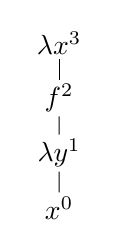
\begin{tikzpicture}[level distance=7mm,inner ysep=0.5mm]
 \node {$\lambda x^3$}
    child {
        node {$f^2$}
        child {
            node {$\lambda y^1$}
            child{
                node{$x^0$}
            }
        }
    };
\end{tikzpicture}
} \noindent \emph{Examples:} Consider the $\beta$-normal term
$\lambda x . f (\lambda y .x)$ where $x,y:o$ and $f:(o,o),o$. The
figure on the right represents the computation tree with the order
of each node in the exponent part. Since node $x$ of order $0$ is
not bound by the order 1 node $\lambda y$, $\tau(M)$ is not
incrementally-bound and by proposition
\ref{prop:Nher_incrbound_and_incrjustified} $\sem{\lambda x . f
(\lambda y .x)}$ is not P-incrementally-justified. Similarly we can
check that $\sem{f (\lambda y .x)}$ is not P-incrementally-justified
whereas $\sem{\lambda y. x}$ is. Also, for any higher-order variable
$x:A$ the computation tree $\tau(x)$ is incrementally-bound
therefore the projection strategies $\pi_i$ are
P-incrementally-justified. From these examples we observe that
application does not preserve P-incremental-justification ($\sem{f}$
and $\sem{\lambda y. x}$ are P-incrementally-justified whereas
$\sem{f (\lambda y .x)}$ is not).
\smallskip

These examples suggest that P-incremental-justification is not a
compositional property. In Chapter \ref{chap:pincrjust} we will
identify a sufficient condition guaranteeing that the composition of
two P-incrementally-justified strategies gives a
P-incrementally-justified strategy. \smallskip


Putting Corollary \ref{cor:Nher_incrbound_iff_incrjustified} and
Lemma \ref{lem:incrbound_iff_etanf_safe} together gives us a
game-semantic characterization of safe terms:
\begin{corollary}[P-incrementally-justified strategies characterize safe closed $\eta\beta$-normal terms]
Let $\Gamma \vdash M : T$ be a simply-typed term (without
interpreted constants). Then:
$$ \sem{\Gamma \vdash M : T} \mbox{ is P-i.j.\ if and only if the $\eta$-long $\beta$-normal form of $M$ is safe.} $$
\end{corollary}



\begin{theorem}[P's pointers are superfluous for safe terms]
\label{thm:safe_ptr_recoverable} Pointers emanating from P-moves in the game semantics of
safe terms are uniquely recoverable.
\end{theorem}
\begin{proof}
Let $M$ be a safe simply-typed term. Then the $\beta$-normal form of
$M$ is also safe, thus by lemma \ref{lem:incrbound_iff_etanf_safe}
(i), $\tau(\betanf{M})$ is incrementally-bound and by proposition
\ref{prop:Nher_incrbound_and_incrjustified}, $\sem{\Gamma \vdash
\betanf{M} :T}$ is a P-incrementally-justified strategy. By lemma
\ref{lem:incrjustified_pointers_uniqu_recover}, P's pointers in
$\sem{\Gamma \vdash \betanf{M} :T}$ are uniquely recoverable.
Finally, the soundness of the game model gives $\sem{\Gamma \vdash
M:T} = \sem{\Gamma \vdash \betanf{M} : T}$.
\end{proof}


\section{Safe PCF and Safe Idealized Algol}

Safe Idealized Algol, or safe \ialgol\ for short, is Idealized Algol
where the application and abstraction rules are restricted the same
way as in the safe $\lambda$-calculus (see rules of section
\ref{sec:safe_nonhomog}).

The properties of the safe $\lambda$-calculus can be transposed
straightforwardly to safe \ialgol. In particular, it can be shown
that safety is preserved by $\beta$-reduction and that no variable
capture occurs when performing substitution on a safe term.

A natural question to ask is whether we can extend the result about
game semantics of safe $\lambda$-terms to safe \ialgol-terms. In
this section we lay out the key elements permitting to prove that
the pointers in the game semantics of safe IA terms can be recovered
uniquely.

Such result has potential applications in algorithmic game semantics.
For instance, by following the framework of \cite{ghicamccusker00},
it may be possible to give a characterisation of the game semantics
of some higher-order fragments of safe \ialgol\ using extended
regular expressions. Subsequently, this would lead to the
decidability of program equivalence for the considered fragment.


\subsection{Formation rules of Safe \ialgol}
We call safe \ialgol\ term any term that is typable within the
following system of formation rules:
$$ \rulename{var} \   \rulef{}{x : A\vdash x : A}
%\qquad  \rulename{const} \   \rulef{}{\vdash f : A} \quad f \in \Sigma
\qquad  \rulename{wk} \   \rulef{\Gamma \vdash M : A}{\Delta \vdash
M : A} \quad  \Gamma \subset \Delta$$

$$ \rulename{app} \  \rulef{\Gamma \vdash M : (A,\ldots,A_l,B)
                                        \qquad \Gamma \vdash N_1 : A_1
                                        \quad \ldots \quad \Gamma \vdash N_l : A_l  }
                                   {\Gamma  \vdash M N_1 \ldots N_l : B}
                                    \quad
\mbox{\fbox{$\forall y \in \Gamma : \ord{y} \geq \ord{B}$}}$$

$$ \rulename{abs} \   \rulef{\Gamma \union \overline{x} : \overline{A} \vdash M : B}
                                   {\Gamma  \vdash \lambda \overline{x} : \overline{A} . M : (\overline{A},B)} \quad
\mbox{\fbox{$\forall y \in \Gamma : \ord{y} \geq \ord(\overline{A},B)$}}$$

$$ \rulename{num} \rulef{}{\Gamma \vdash n :\texttt{exp}}
\qquad \rulename{succ} \rulef{\Gamma \vdash M:\texttt{exp} }{\Gamma
\vdash \texttt{succ}\ M:\texttt{exp}} \qquad \rulename{pred}
\rulef{\Gamma \vdash M:\texttt{exp} }{\Gamma \vdash \texttt{pred}\
M:\texttt{exp}}$$

$$
\rulename{cond} \rulef{\Gamma \vdash M : \texttt{exp} \qquad \Gamma
\vdash N_1 : \texttt{exp} \qquad \Gamma \vdash N_2 : \texttt{exp}
}{\Gamma \vdash \texttt{cond}\ M\ N_1\ N_2} \qquad  \rulename{rec}
\rulef{\Gamma \vdash M : A\rightarrow A }{ \Gamma \vdash Y_A M :
A}$$

$$ \rulename{seq} \rulef{\Gamma \vdash M : \texttt{com} \quad \Gamma \vdash N :A}
    {\Gamma \vdash \texttt{seq}_A \ M\ N\ : A} \quad A \in \{ \texttt{com}, \texttt{exp}\}$$

$$ \rulename{assign} \rulef{\Gamma \vdash M : \texttt{var} \quad \Gamma \vdash N : \texttt{exp}}
    {\Gamma \vdash \texttt{assign}\ M\ N\ : \texttt{com}}
\qquad
 \rulename{deref} \rulef{\Gamma \vdash M : \texttt{var}}
    {\Gamma \vdash \texttt{deref}\ M\ : \texttt{exp}}$$

$$ \rulename{new} \rulef{\Gamma, x : \texttt{var} \vdash M : A}
    {\Gamma \vdash \texttt{new } x \texttt{ in } M} \quad A \in \{ \texttt{com}, \texttt{exp}\}$$

$$ \rulename{mkvar} \rulef{\Gamma \vdash M_1 : \texttt{exp} \rightarrow \texttt{com} \quad \Gamma \vdash M_2 : \texttt{exp}}
    {\Gamma \vdash \texttt{mkvar } M_1\ M_2\ : \texttt{var}}$$

\subsection{Small-step semantics of Safe \ialgol}
In the first chapter we defined the operational semantics of
\ialgol\ using a big step semantics. The operational semantics of
\ialgol\ can be defined equivalently using a small-step semantics.
The reduction rules of the small-step semantics are of the form $s,e
\rightarrow s',e'$ where $s$ and $s'$ denotes the stores and $e$ and
$e'$ denotes \ialgol\ expressions.

Let us give the rules that tell how to reduce redexes:
\begin{itemize}
\item the reduction of safe-redex (relation $\beta_s$ from definition \ref{dfn:safereduction});
\item reduction rules for \pcf\ constants:
\begin{eqnarray*}
\pcfsucc\ n &\rightarrow& n+1 \\
\pcfpred\ n+1 &\rightarrow& n \\
\pcfpred\ 0 &\rightarrow& 0 \\
\pcfcond\ 0\ N_1 N_2 &\rightarrow& N_1 \\
\pcfcond\ n+1\ N_1 N_2 &\rightarrow& N_2 \\
Y\ M &\rightarrow& M (Y M)
\end{eqnarray*}
\item reduction rules for \ialgol\ constants:
\begin{eqnarray*}
\iaseq\ \iaskip\  M &\rightarrow& M \\
s, \ianewin{x}\ M &\rightarrow& (s|x\mapsto 0), M \\
s, \iaassign\ x\ n &\rightarrow& (s|x\mapsto n), \iaskip \\
s, \iaderef\ x &\rightarrow& s, s(x) \\
\iaassign\ (\iamkvar M N)\ n &\rightarrow& M n \\
\iaderef\ (\iamkvar M N) &\rightarrow& N
\end{eqnarray*}
\end{itemize}

Redex can also be reduced when they occur as subexpressions within a
larger expression. We make use of evaluation contexts to indicate
when such reduction can happen. Evaluation contexts are given by the
following grammar:
\begin{eqnarray*}
E[-] &::=& - |\ E N\ |\ \pcfsucc\ E\ |\ \pcfpred\ E\ |\ \pcfcond\ E\ N_1\ N_2\ |\ \\
&&    \iaseq\ E\ N\ |\ \iaderef\ E\ |\ \iaassign\ E\ n\ |\ \iaassign\ M\ E \ |\ \\
&&    \iamkvar\ M\ E\ |\ \iamkvar\ E\ M\ |\ \ianewin{x}\ E  .
\end{eqnarray*}

The small-step semantics is completed with following rule:
$$ \rulef{M \rightarrow N}{E[M] \rightarrow E[N]} $$

\begin{lemma}[Reduction preserves safety]
\label{lem:ia_safety_preserved} Let $M$ be a safe IA term. If
$M \rightarrow N$ then $N$ is also a safe term.
\end{lemma}
This can be proved easily by induction on the structure of M.


\subsection{Safe \pcf\ fragment}
In this section, we show how to extend the results obtained for the
safe $\lambda$-calculus to the \pcf\ fragment of safe \ialgol.

The $Y$ combinator needs a special treatment. In order to deal with
it, we follow the idea of \cite{abramsky:game-semantics-tutorial}:
we consider the sublanguage $\pcf_1$ of \pcf\ in which the only
allowed use of the $Y$ combinator is in terms of the form $Y(
\lambda x:A .x )$ for some type $A$. We will write $\Omega_A$ to
denote the non-terminating term $Y(\lambda x:A .x)$ for a given type
$A$.

We introduce the \emph{syntactic approximants} to $Y_A M$:
\begin{eqnarray*}
Y^0_A M &=& \Gamma \vdash \Omega_A : A\\
Y^{n+1}_A M &=& M( Y^n M )
\end{eqnarray*}
For any \pcf\ term $M$ and natural number $n$, we define $M_n$ to be
the $\pcf_1$ term obtained from $M$ by replacing each subterm of the
form $Y N$ with $Y^n N_n$. We have $\sem{M} = \Union_{n\in\omega}
\sem{M_n}$ (\cite{abramsky:game-semantics-tutorial}, lemma 16).


\subsubsection{Computation tree}

We would like to define a unique computation tree for terms that use
the $Y$ combinator.

Let us first define the computation tree for $\pcf_1$ terms. We
introduce a special $\Sigma$-constant $\bot$ representing the
non-terminating computation of ground type $\Omega_o$. Given any
type $A = (A_1, \ldots, A_n, o)$, the computation tree
$\tau(\Omega_A)$ is defined to be the tree representation of
$\lambda x_1:A_1 \ldots x_n:A_n . \bot$. The computation tree of a
$\pcf_1$ term is then computed inductively in the standard way.

We now introduce a partial order on the set of computation trees.

A \emph{tree} $t$ is a labelling function $t:T\rightarrow L$ where
$T$, called the domain of $t$ and written $dom(t)$, is a non-empty
prefix-closed subset of some free monoid $X^*$ and $L$ denotes the
set of possible labels. Intuitively, $T$ represents the structure of
the tree (the set of all paths) and $t$ is the labelling function
mapping paths to labels. Trees can be ordered using the
\emph{approximation ordering} defined in \cite{KNU02}, section 1: we
write $t' \sqsubseteq t$ if the tree $t'$ is obtained from $t$ by
replacing some of its subtrees by $\bot$. Formally:
$$t' \sqsubseteq t \quad \iff dom(t') \subseteq dom(t) \wedge \forall  w \in dom(t'). (t'(w) = t(w) \vee t'(w) = \bot).$$
The set of all trees together with the approximation ordering is a
complete partial order.

We now consider a strict subset of the set of all trees: the set of
computation trees. A computation tree is a tree which represents the
$\eta$-normal form of some (potentially infinite) \pcf\ term. In
other words a tree is a computation tree if it can be written
$\tau(M)$ for some infinite \pcf\ term $M$. The set $L$ of labels is
constituted of the $\Sigma$-constants, @, the special constant
$\bot$, variables and abstractions of any sequence of variables. We
will write $(CT, \sqsubseteq)$ to denote the set of computation
trees ordered by the approximation ordering $\sqsubseteq$ defined
above. $(CT, \sqsubseteq)$ is also a complete partial order.

It is easy to check that the sequence of computation trees
$(\tau(M_n))_{n\in\omega}$ is a chain. We can therefore define the
computation tree of a \pcf\ term $M$ to be the least upper-bound of
the chain of computation trees of its approximants:
$$\tau(M) = \Union_{n\in\omega}(\tau(M_n))_{n\in\omega}.$$

In other words, we construct the computation tree by expanding
infinitely any subterm of the form $Y M$. For instance consider the
term $M = Y (\lambda f x. f x)$ where $f:(o,o)$ and $x:o$. Its
computation tree $\tau(M)$, represented below, is a tree
representation of the $\eta$-normal form of the infinite term
$(\lambda f x. f x) ((\lambda f x. f x) ((\lambda f x. f x)  (
\ldots$.
$$\tau(M) =
\begin{tikzpicture}[level distance=7mm,inner ysep=0.5mm,baseline=(root.base)]
\node (root) {$\lambda y$}
child {
    node {@}
    child {
        node {$\lambda f x$}
        child{
            node{$f$}
            child{
                node{$\lambda$}
                child{
                    node{$x$}
                }
            }
        }
    }
    child{
        node{$\tau(M)$}
    }
    child{
        node{$\lambda$}
        child{
            node{$y$}
        }
    }
};
\end{tikzpicture}
$$
The remaining operators of \ialgol\ are treated as standard
constants and the corresponding computation tree is constructed from
the $\eta$-normal form of the term in the standard way. For instance
the diagram below shows the computation tree for $\pcfcond\ b\ x\ y$
(left) and $\lambda x . 5$ (right):
$$\begin{tikzpicture}[level distance=7mm,inner ysep=0.5mm,baseline=(root.base)]
\path
node (root) {$\lambda b x y$}
child {
    node {\pcfcond}
    child {
        node {$\lambda$}
        child{
            node{$b$}
        }
    }
    child{
        node {$\lambda$}
        child{
            node{$x$}
        }
    }
    child{
        node {$\lambda$}
        child{
            node{$y$}
        }
    }
}
+(4,0)
node {$\lambda$}
child{
    node{$5$}
};
\end{tikzpicture}
$$
The node labelled $5$ has, like any other node, children
value-leaves which are not represented on the diagram above for
simplicity.

\subsubsection{Traversal}

New traversal rules accompany the additional constants of \ialgol.
There is one additional rule for natural number constants:
\begin{itemize}
\item (Nat) If $t \cdot n$ is a traversal where $n$ denotes a node labelled with some numeral constant $i\in \nat$ then
            $\Pstr{t \cdot (n){n} \cdot (in-n){i_n}}$
            is also a traversal where $i_n$ denotes the value-leaf of $m$ corresponding to the value $i\in \nat$.
\end{itemize}

\noindent The traversals rules for \pcfpred\ and \pcfsucc\ are
defined similarly. For instance, the rules for \pcfsucc\ are:
\begin{itemize}
\item (Succ) If $t \cdot \pcfsucc$ is a traversal and $\lambda$ denotes the only child node of \pcfsucc\ then
$\Pstr{t \cdot (succ){\pcfsucc} \cdot (l-succ,35:1){\lambda}}$ is also a traversal.

\item (Succ') If
$\Pstr{ t_1 \cdot (succ){\pcfsucc} \cdot (l-succ,35:1){\lambda} \cdot t_2
\cdot (lv-l){i_{\lambda}}} $ is a traversal for some
$i \in \nat$ then $\Pstr{t_1 \cdot (succ){\pcfsucc} \cdot
(l-succ,35:1){\lambda} \cdot t_2 \cdot (lv-l){i_{\lambda}} \cdot
(succv-succ,25){(i+1)_{\pcfsucc}}}$ is also a traversal.
\end{itemize}

\noindent In the computation tree, nodes labelled with \pcfcond\
have three children nodes numbered from $1$ to $3$ corresponding to
the three parameters of the operator \pcfcond. The traversal rules
are:
\begin{itemize}
\item (Cond-If) If $t_1 \cdot \pcfcond$ is a traversal and $\lambda$ denotes the first child of \pcfcond\ then
$\Pstr{ t_1 \cdot (cond){{\pcfcond}} \cdot (l-cond,30:1){\lambda}}$
 is also a traversal.

\item (Cond-ThenElse) If
$\Pstr{t_1 \cdot (cond){\pcfcond} \cdot (l-cond,35:1){\lambda} \cdot t_2
\cdot (lv-l){i_{\lambda}}} $
then $\Pstr{t_1 \cdot
(cond){\pcfcond} \cdot (l-cond,35:1){\lambda} \cdot t_2 \cdot
(lv-l){i_{\lambda}} \cdot (condthenelse-cond,35:{2+[i>0]}){\lambda} }
$
is also a traversal.



\item (Cond') If
$\Pstr{t_1 \cdot (cond){\pcfcond} \cdot t_2 \cdot (l-cond,35:k){\lambda}
\cdot t_3 \cdot (lv-l){i_{\lambda}}}$
 for $k=2$ or $k=3$ then  $\Pstr{ t_1 \cdot
(cond){\pcfcond} \cdot t_2 \cdot (l-cond,35:k){\lambda} \cdot t_3
\cdot (lv-l){i_{\lambda}} \cdot (condv-cond,25){i_{\pcfcond}}}$
 is also a traversal.
\end{itemize}
It is easy to verify that these traversal rules are all
well-behaved. This completes the definition of traversal for the
\pcf\ subset of \ialgol.

\subsubsection{Interaction semantics}
We recall that the definition of the syntactically-revealed
semantics (Sec.\ \ref{sec:interaction_semantics}, Def.\
\ref{dfn:fully_revealed_semantics}) accounts for the presence of
interpreted constants: For any $\Sigma$-constant $f :
(A_1,\ldots,A_p,B)$ in the language, the revealed strategy of a term
of the form $\lambda \overline{\xi}. f N_1 \ldots N_p$ is defined
as:
$$ \revsem{\lambda \overline{\xi}. f N_1 \ldots N_p} = \langle \revsem{N_1}, \ldots, \revsem{N_p} \rangle \fatsemi^{0..p-1} \sem{f}.$$
where $\sem{f}$ is the standard strategy denotation of $f$.

\subsubsection{Correspondence theorem}
We would like to prove the counterpart of proposition
\ref{prop:rel_gamesem_trav} in the context of the simply-typed
$\lambda$-calculus \emph{with interpreted PCF constants}. The game
model of the language \pcf\ is given by the category $\mathcal{C}_b$
of well-bracketed strategies. Hence the well-bracketing assumption
stated at the beginning of section \ref{sec:gamesemcorresp} is
satisfied.

We first prove that $\travset(\_)^{\filter \theroot}$ is continuous.
\begin{lemma}
\label{lem:travred_continuous} Let $(S,\subseteq)$ denote the set of
sets of justified sequences of nodes ordered by subset inclusion.
The function $\travset(\_)^{\filter \theroot} : (CT,\sqsubseteq)
\rightarrow (S,\subseteq)$ is continuous.
\end{lemma}
\begin{proof} \
    \begin{description}
    \item[Monotonicity:] Let $T$ and $T'$ be two computation trees such that $T \sqsubseteq T'$
    and let $t$ be some traversal of $T$.
    Traversals ending with a node labelled $\bot$ are maximal therefore $\bot$ can only occur
    at the last position in a traversal. Let us prove the following two properties:
        \begin{itemize}
            \item[(i)]  If $t = t \cdot n$ with $n\neq \bot$ then $t$ is a traversal of $T'$;
            \item[(ii)] if $t= t_1 \cdot \bot$ then $t_1\in \travset(T')$.
        \end{itemize}

        (i) By induction on the length of $t$. It is trivial for the empty traversal.
            Suppose that $t = t_1 \cdot n$ is a traversal with $n \neq \bot$.
            By the induction hypothesis, $t_1$ is a traversal of $T'$.

            We observe that for all traversal rules, the traversal produced is of the form $t_1 \cdot n$ where
            $n$ is defined to be a child node or value-leaf of some node $m$ occurring in $t_1$.
            Moreover, the choice of the node $n$ only depends on the traversal $t_1$
            (for the constant rules, this is guaranteed by assumption (WB)).

            Since $T \sqsubseteq T'$, any node $m$ occurring in $t_1$ belongs
            to $T'$ and the children nodes and leaves of $m$ in $T$ also belong to the tree $T'$.
            Hence $n$ is also present in $T'$ and the rule used to produce the traversal $t$ of $T$
            can be used to produce the traversal $t$ of $T'$.

        (ii) $\bot$ can only occur at the last position in a traversal
        therefore $t_1$ does not end with $\bot$ and by (i) we have $t_1\in \travset(T')$.
\vspace{6pt}

        Hence we have:
        \begin{align*}
        \travset(T)^{\filter \theroot} &= \{ t \filter r \ | \ t \in \travset(T)     \} \\
        & = \{ (t\cdot n) \filter r \ | \ t\cdot n \in \travset(T) \wedge n \neq \bot \}
            \union \{ (t \cdot \bot ) \filter r \ | \ t \cdot \bot \in \travset(T)  \} \\
\mbox{(by (i) and (ii))} \quad        & \subseteq  \{ (t\cdot n)
\filter r \ | \ t\cdot n \in \travset(T') \wedge n \neq \bot
\}
            \union \{ t \filter r \ | \ t \in \travset(T')  \} \\
        & = \travset(T')^{\filter \theroot}
        \end{align*}

        \item[Continuity:] Let $t \in \travset \left( \Union_{n\in\omega} T_n \right)$.
        We write $t_i$ for the finite prefix of $t$ of length $i$.
        The set of traversals is prefix-closed therefore $t_i \in \travset \left( \Union_{n\in\omega} T_n \right)$ for any $i$.
        Since $t_i$ has finite length we have $t_i \in \travset(T_{j_i})$ for some $j_i \in \omega$.
        Therefore we have:
        \begin{align*}
          t \filter r &= (\bigvee_{i\in\omega} t_i ) \filter r   & (\mbox{the sequence $(t_i)_{i\in\omega}$ converges to $t$}) \\
          &= \Union_{i\in\omega} ( t_i \filter r )   & (\_ \filter r \mbox{ is continuous, lemma \ref{lem:projection_continuous}}) \\
          &\in \Union_{i\in\omega} \travset(T_{j_i})^{\filter \theroot}   & (t_i \in \travset(T_{j_i})) \\
          &\subseteq \Union_{i\in\omega} \travset(T_i)^{\filter \theroot}   & (\mbox{since } \{ j_i \sthat i \in \omega \} \subseteq \omega)
        \end{align*}

        Hence $\travset(\Union_{n\in\omega} T_n )^{\filter
        \theroot} \subseteq \Union_{n\in\omega}
        \travset(T_n)^{\filter \theroot}.$

    \end{description}
\end{proof}

\begin{proposition}
Let $\Gamma \vdash M : T$ be a PCF term and $r$ be the root of
$\tau(M)$. Then:
\begin{align*}
(i)  \quad\varphi_M(\travset(M)^*) = \revsem{M},  \\
(ii) \quad \varphi_M(\travset(M)^{\filter \theroot}) = \sem{M}.
\end{align*}
\end{proposition}
\begin{proof}
We first prove the result for $\pcf_1$: (i) The proof is an
induction identical to the proof of proposition
\ref{prop:rel_gamesem_trav}. However we need to complete the case
analysis with the $\Sigma$-constant cases:
\begin{itemize}
\item The cases \pcfsucc, \pcfpred, \pcfcond\ and numeral constants are straightforward.

\item Suppose $M = \Omega_o$ then $\travset(\Omega_o) = \prefset ( \{ \lambda \cdot \bot \} )$ therefore
$\travset(\Omega_o)^{\filter \theroot} = \prefset( \{ \lambda \}
)$ and $\sem{\Omega_o} = \prefset( \{ q \})$ with
$\varphi(\lambda) = q$. Hence $\sem{\Omega_o} = \varphi
(\travset(\Omega_o)^{\filter \theroot})$.
\end{itemize}
(ii) is a direct consequence of (i) and the Projection Lemma
\ref{lem:varphi_proj}. \vspace{10pt}

\noindent We now extend the result to \pcf. Let $M$ be a \pcf\ term,
we have:
\begin{align*}
\sem{M} &= \Union_{n\in\omega} \sem{M_n} & (\mbox{\cite{abramsky:game-semantics-tutorial}, lemma 16})\\
&= \Union_{n\in\omega} \travset(\tau(M_n))^{\filter \theroot} & (M_n \mbox{ is a $\pcf_1$ term}) \\
&= \travset(\Union_{n\in\omega} \tau(M_n) )^{\filter \theroot} & (\mbox{by continuity of $\travset(\_)^{\filter \theroot}$, lemma \ref{lem:travred_continuous}}) \\
&= \travset(\tau(M))^{\filter \theroot} & (\mbox{by definition of } \tau(M)) \\
&= \travset(M)^{\filter \theroot} & (\mbox{abbreviation}).
\end{align*}
\end{proof}

Hence by corollary \ref{cor:varphi_bij}, $\varphi$ defines a
bijection from $\travset(M)^{\filter \theroot}$ to $\sem{M}$:
$$\varphi : \travset(M)^{\filter \theroot} \stackrel{\cong}{\longrightarrow} \sem{M}.$$

\subsubsection{First example: the successor operator}

Consider the term $M = \pcfsucc\ 5$ whose computation tree is
represented below. The value-leaves are also represented on the
diagram, they are the vertices attached to their parent node with a dashed line.
\begin{center}
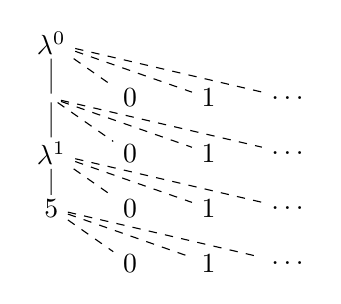
\begin{tikzpicture}[level distance=7mm,inner ysep=0.5mm,sibling distance=10mm]
\node {$\lambda^0$}
    child[missing]{}
    child[missing]{}
    child[missing]{}
    child {
        node {\pcfsucc}
        child[missing]{}
        child[missing]{}
        child[missing]{}
        child {
            node {$\lambda^1$}
            child[missing]{}
            child[missing]{}
            child[missing]{}
            child{
                node{$5$}
                child[missing]{}
                child[missing]{}
                child[missing]{}
                child[missing]{}
                child{node{$0$} edge from parent[dashed]}
                child{node{$1$} edge from parent[dashed]}
                child{node{$\ldots$} edge from parent[dashed]}
            }
            child{node{$0$} edge from parent[dashed]}
            child{node{$1$} edge from parent[dashed]}
            child{node{$\ldots$} edge from parent[dashed]}
        }
        child{node{$0$} edge from parent[dashed]}
        child{node{$1$} edge from parent[dashed]}
        child{node{$\ldots$} edge from parent[dashed]}
    }
    child{node{$0$} edge from parent[dashed]}
    child{node{$1$} edge from parent[dashed]}
    child{node{$\ldots$} edge from parent[dashed]}
;
\end{tikzpicture}
\end{center}

The following sequence of nodes is a traversal of $\tau(M)$:
$$ \Pstr[20pt]{ t = (l0){\lambda^0} \cdot (succ){\pcfsucc} \cdot (l1){\lambda^1} \cdot (c5){5} \cdot (v55-c5){5_5} \cdot (5l1-l1){5_{\lambda^1}} \cdot (6succ-succ){6_\pcfsucc} \cdot (6l0-l0,35){6_{\lambda^0}}}.
$$

The subsequences $t^*$ and $t \filter r$ are given by:
$$
\Pstr[17pt]{ t^* = (l0){\lambda^0} \cdot (l1-l0){\lambda^1} \cdot
(5l1-l1){5_{\lambda^1}} \cdot (6l0-l0){6_{\lambda^0}}.
\qquad  \mbox{ and } \qquad t
\filter r = (l0b){\lambda^0} \cdot
(6l0b-l0b){6_{\lambda^0}}. }
$$
We have $\varphi(t^*) = q_0 \cdot q_5 \cdot 5_{q_5} \cdot 5_{q_0}$
and $\varphi(t\filter r) = q_0 \cdot 5_{q_0}$ where $q_0$
and $q_5$ denote the roots of two flat arenas over $\nat$. These two
sequences of moves correspond to some play of the interaction
semantics and the standard semantics respectively. The interaction
play is represented below:
\begin{center}
\begin{tikzpicture}[style={anchor=base}]
\matrix (m) [matrix of math nodes]
{
\textbf{1} & \stackrel{5}{\longrightarrow} & \nat & \stackrel{\pcfsucc}{\longrightarrow} & \nat \\
&&&&  \node(q0){q_0}; \\
&&  \node(q5){q_5}; \\
&&  \node(a5){5_{q_5}}; \\
&&&&  \node(a6){6_{q_0}}; \\
};
\path (q5) edge[tableptr] (q0); 
\draw[tableptr] (a5.west) .. controls +(160:0.2cm) and +(220:0.2cm) .. (q5.west);
\draw (a6) edge[tableptr] (q0);
\end{tikzpicture}
\end{center}

\subsubsection{Second example: the conditional operator}

\piccaption{The computation tree of the term $\lambda x y . \pcfcond\ 1\ x\ y$.}
\parpic[l]{
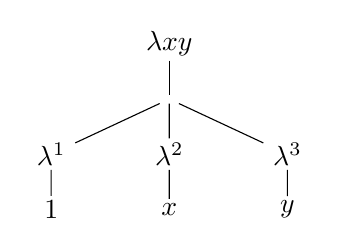
\begin{tikzpicture}[level distance=7mm,inner ysep=0.5mm,baseline=(root.base)]
\path
node (root) {$\lambda x y$}
child {
    node {\pcfcond}
    child {
        node {$\lambda^1$}
        child{
            node{$1$}
        }
    }
    child{
        node {$\lambda^2$}
        child{
            node{$x$}
        }
    }
    child{
        node {$\lambda^3$}
        child{
            node{$y$}
        }
    }
};
\end{tikzpicture}
}
Take the computation tree represented on the left (value-leaves are not shown). For any value $v \in\mathcal{D}$ the following sequence of nodes is a traversal:
$$\Pstr[27pt]{ t = (lxy){\lambda x y} \cdot (cond){\pcfcond} \cdot (l1-cond){\lambda^1} \cdot (1){1} \cdot (v11-1){1_1}
    \cdot (l3){\lambda^3} \cdot (y-lxy){y} \cdot (vy-y){v_y}  \cdot (vl3-l3){v_{\lambda^3}} \cdot (vcond-cond,30){v_{\pcfcond}}
    \cdot (vlxy-lxy,30){v_{\lambda x y}}.
}
$$
The subsequence $t^*$ and the reduction $t \filter\theroot$ are:
$$
\Pstr[17pt]{ t^* =  (lxy){\lambda x y} \cdot
        (l1-lxy){\lambda^1} \cdot
        (l3-lxy){\lambda^3} \cdot
        (y-lxy){y} \cdot
        (vy-y){v_y}  \cdot
        (vl3-l3){v_{\lambda^3}} \cdot
        (vlxy-lxy,35){v_{\lambda x y}}
\qquad  \mbox{ and } \qquad t \filter\theroot =
(lxyb){\lambda x y} \cdot (yb-lxyb){y} \cdot (vyb-yb){v_y}
\cdot (vlxyb-lxyb){v_{\lambda x y}}.
}
$$
The correspondence theorem tells us that the sequence of moves $\varphi(t^*)$ (represented in the diagram below) is a play of the
revealed semantics, and the sequence $\varphi(t\filter\theroot)$
is a play of the standard semantics that is obtained by hiding the internal moves from $\varphi(t^*)$.

\begin{center}
\begin{tikzpicture}[style={anchor=base}]
  \matrix[matrix of math nodes]
  {
  \nat & \times & \nat & \stackrel{\sigcol{\langle \sem{1}, \pi_1, \pi_2\rangle}}\longrightarrow & \nat & \times & \nat & \times &
\nat & \stackrel{\mucol\pcfcond}\longrightarrow & \nat \\
&&&&&&&&&&  \node(q0){q_0^{(\lambda x y)}}; \\
&&&&  \node(qa){q_a^{(\lambda^1)}}; \\
&&&&  \node(1){1}; \\
&&&&&&  \node(qb){q_b^{(\lambda^2)}}; \\
&&  \node(qy){q_y^{(y)}}; \\
&&  \node(vqy){v_{q_y}}; \\
&&&&&&  \node(vqb){v_{q_b}}; \\
&&&&&&&&&& \node(vq0){v_{q_0}}; \\
};
\path (vq0) edge[tableptr] (q0);
\path (vqb) edge[tableptr] (qb);
\draw[->] (vqy.west) .. controls +(160:0.2cm) and +(220:0.2cm) .. (qy.west);
\path (qy) edge[tableptr] (qb);
\path (qb) edge[tableptr] (q0);
\draw[->] (1.west) .. controls +(160:0.2cm) and +(200:0.2cm) .. (qa.west);
\path (qa) edge[tableptr] (q0);
\end{tikzpicture}
\end{center}

\subsubsection{Game characterisation of safe terms}

A difficulty arises because of the presence of the Y combinator :
computation trees of \pcf\ terms are potentially infinite. Despite
this particularity, lemma \ref{lem:incrbound_iff_etanf_safe} still
holds in the \pcf\ setting:
\begin{lemma} \label{lem:pcf_safe_imp_incrbound} If $M$ is a safe
PCF term then $\tau(M)$ is incrementally-bound.
\end{lemma}
\begin{proof}
Let $i$ denote the number of occurrences of the Y combinator in $M$.
We first prove by induction on $i$ that $M_k$ is safe for any $k\in
\omega$. \emph{Base case:} $i=0$ then $M_k = M$. \emph{Step case:}
$i>0$. Let $Y_A N$ be a subterm of $M$. Since $M$ is safe, $N$ is
also safe. The number of occurrences of the Y combinator in $N$ is
smaller than $i$ therefore by the induction hypothesis $N_k$ is
safe. Consequently the term $Y_A^k N_k = \underbrace{N_k ( \ldots (
N_k}_{k \mbox{ times}} \Omega ) \ldots )$ is also safe and by
compositionality so is $M_k$.

Clearly, lemma \ref{lem:incrbound_iff_etanf_safe}(i) is remains
valid for infinite $\pcf_1$ terms (the subterms of the form $\Omega$
are just represented by the constant $\bot$ in the computation
tree), thus since $M_k$ is a safe $\pcf_1$ term, $\tau(M_k)$ is
incrementally-bound. Now let $z$ be a variable node in $\tau(M) =
\Union_{k\in\omega} \tau(M_k)$. There exists $k\in \omega$ such that
$z$ belongs to $\tau(M_k) \sqsubseteq \tau(M)$. If we write $r_k$ to
denote the root of the tree $\tau(M_k)$ then the path $[r_k,z]$ in
$\tau(M_k)$ is equal to the path $[r,z]$ in $\tau(M)$. Hence, since
the node $z$ is incrementally-bound in $\tau(M_k)$, it is also
incrementally-bound in $\tau(M)$.
\end{proof}


\begin{theorem}
Safe PCF terms are denoted by P-incrementally-justified strategies.
\end{theorem}
\begin{proof}
Let $M^{\infty}$ be the $\beta$-normal form of $M$ (i.e. the possibly infinite term obtained by reducing all the redexes in $M$). By lemma \ref{lem:ia_safety_preserved}, safety is preserved by small-step reduction therefore, by lemma \ref{lem:pcf_safe_imp_incrbound}, if $M$ is a \pcf\ term then $\tau(M^{\infty})$ is also
incrementally-bound.

Since \pcf\ constant rules are well-behaved (by Lemma
\ref{lem:sigma_order1_are_wellbehaved}), the result from Lemma
\ref{lem:betanf_wellbehavedconst_trav_pview_red} is also true for
Safe \pcf. Thus proposition
\ref{prop:Nher_incrbound_and_incrjustified}(i) remains valid for the
infinite computation trees of \pcf: infinite terms in $\beta$-nf
with an incrementally-bound computation tree are denoted by
P-incrementally-justified strategies. Consequently,
$\sem{M^{\infty}}$ is P-incrementally-justified. By soundness of the
game denotation, $\sem{M^{\infty}} = \sem{M}$, thus $\sem{M}$ is
P-incrementally-justified.
\end{proof}

Consequently, P-pointers are superfluous in the game denotation of safe \pcf\ terms {\it i.e.} pointers emanating from P-moves are uniquely recoverable.

\subsection{Safe \ialgol}

We are now in a position to consider the full safe Idealized Algol
language. The general idea is the same as for safe \pcf, however
there are some difficulties caused by the presence of the two new
base types \iavar\ and \iacom. We just give indications on how to
adapt our framework to the particular case of safe \ialgol\ without
giving the complete proofs. However we believe that enough
indications are given to convince the reader that the argument used
in the \pcf\ case can be easily adapted to \ialgol.

\subsubsection{Computation DAG}
Crucially, all the languages that we have considered up to now (lambda calculus and \pcf) do not have product types. Consequently, the arenas involved in their game model only have a single initial move at most, and therefore they can be
regarded as trees. This had permitted us to represent the game denotation of term directly on some representation of its abstract syntax tree. In \ialgol, however, the type \iavar\ is given by the product $\iacom^{\nat} \times \iaexp$. Therefore the corresponding game has an infinite number of initial moves. But tree structures such as the AST of the term have only one root therefore we have to find a different way to represent the game semantics.

The solution consists in using \emph{computation directed acyclic graphs} (DAG) instead of computation trees. The computation DAG is an abstract graph representation of the syntax of the term.
It can have (possibly infinitely) many roots, and any two nodes in the same level can share children at the next level.

\emph{Notations:} For any type $\mu$, we write
$\mathcal{D}_\mu$ to denote the set of values of type $\mu$.
We have $\mathcal{D}_{\iaexp} = \nat$,
$\mathcal{D}_{\iacom} = \{ \iadone \}$
and $\mathcal{D}_{\iavar} = \mathcal{D}_{\iaexp} \union \mathcal{D}_{\iacom}$. For any node $n$, if $\kappa(n)$ is of type $(A_1,\ldots A_n,B)$, we call $B$ the \emph{return type of $n$}. The set of value-leaves of a node $n$ is given by $\mathcal{D}_{\mu}$ where $\mu$ is the return type of $n$.
For conciseness, when representing value-leaves in the DAG, we merge all the value-leaves of a given node of type $\mu$ into a single leaf labelled $\mathcal{D}_\mu$.

For instance the tree
\begin{center}
\begin{tikzpicture}[level distance=7mm,inner ysep=0.5mm,baseline=(root.base),sibling distance=5mm]
\path
node (root) {$n$}
child {
    node {$\mathcal{D}_\iaexp$}
}
+(1.5,0) node {stands for}
+(3,0)
node {$n$}
    child {node {$0$} }
    child {node {$1$}}
    child {node {$2$}}
    child {node {$\ldots$}}
+(7,0) node {and}
+(8,0)
node {$n$}
child{
    node{$\mathcal{D}_\iacom$}
}
+(9,0) node {for}
+(10,0)
node {$n$}
child{
    node{\iadone}
};
\end{tikzpicture}.
\end{center}

Table \ref{tab:ia_computationdag} shows the computation DAG for each term-construct of \ialgol.

A term of type \iavar\ has a computation DAG with an infinite number of root $\lambda$-nodes. Suppose that $M$ is a term of type \iavar, then the computation DAG for $\lambda \overline{\xi} . M$ is obtained by relabelling the root $\lambda$-nodes $\lambda^r$,
$\lambda^{w_0}$, $\lambda^{w_1}$, $\lambda^{w_2}$, \ldots into
$\lambda^r \overline{\xi}$, $\lambda^{w_0} \overline{\xi}$,
$\lambda^{w_1} \overline{\xi}$, $\lambda^{w_2} \overline{\xi}$,
\ldots. For a term $M$  of type \iaexp\ or \iacom, the computation
DAG for $\lambda \overline{\xi} . M$ is computed in the same way as
in the safe $\lambda$-calculus.

\begin{table}
\begin{center}
\begin{tabular}{lc}
$M$ & $\tau(M)$ \\ \hline \hline \\
\parbox{3cm}{x $: \mu$ \\
$\mu \in \{ \iacom, \iaexp \}$} &

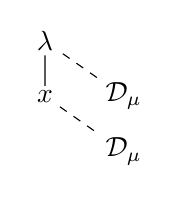
\begin{tikzpicture}[level distance=7mm,inner ysep=0.5mm,sibling distance=10mm]
\node {$\lambda$}
child[missing]{}
child {
    node {$x$}
    child[missing]{}
    child[missing]{}
    child {
        node {$\mathcal{D}_\mu$}
        edge from parent[dashed]
    }
}
child{node{$\mathcal{D}_\mu$} edge from parent[dashed]}
;
\end{tikzpicture}
\\ \\
x : \iavar &
\begin{tikzpicture}
\matrix (m) [matrix of math nodes, row sep=5mm]
{
\lambda^r & \lambda^{w_0} & \lambda^{w_1}  & \lambda^{w_2} & \lambda^{w_{\ldots}} \\
    \mathcal{D}_\iaexp &  & x & & \iadone \\
    &  &  & \mathcal{D}_\iaexp & \iadone \\
};
\draw[-] (m-1-1) -- (m-2-3)
         (m-1-2) -- (m-2-3)
         (m-1-3) -- (m-2-3)
         (m-1-4) -- (m-2-3)
         (m-1-5) -- (m-2-3);
\draw[dashed] (m-2-3) -- (m-3-4)
              (m-2-3) -- (m-3-5)
              (m-1-1) -- (m-2-1)
              (m-1-5) -- (m-2-5)
              (m-1-4) -- (m-2-5)
              (m-1-3) -- (m-2-5)
              (m-1-2) -- (m-2-5);
\end{tikzpicture}   
\\ \\
\iaskip : \iacom &
    \begin{tikzpicture}[level distance=7mm,inner ysep=0.5mm,sibling distance=10mm]
\node {$\lambda$}
child[missing]{}
child {
    node {\iaskip}
    child[missing]{}
    child[missing]{}
    child {
        node {\iadone}
        edge from parent[dashed]
    }
}
child{node{\iadone} edge from parent[dashed]}
;
\end{tikzpicture}
\\ \\
$\iaassign\ L\ N :\iacom$ &
\begin{tikzpicture}[level distance=7mm,inner ysep=0.5mm,sibling distance=20mm]
\node {$\lambda$}
child[missing]{}
child {
    node {\iaassign}
    child{node{$\tau(N:\iaexp)$}}
    child{node{$\tau(L:\iavar)$}}
    child {
        node {\iadone}
        edge from parent[dashed]
    }
}
child{node{\iadone} edge from parent[dashed]};
\end{tikzpicture}
\\ \\
$\iaderef\ L :\iaexp$ &
\begin{tikzpicture}[level distance=7mm,inner ysep=0.5mm,sibling distance=15mm]
\node {$\lambda$}
child[missing]{}
child {
    node {\iaderef}
    child[missing]{}
    child{node{$\tau(L:\iavar)$}}
    child {
        node {\iadone}
        edge from parent[dashed]
    }
}
child{node{\iadone} edge from parent[dashed]}
;
\end{tikzpicture}
\\ \\
\parbox{3cm}{$\iaseq_{\mu}\ N_1\ N_2 :\iacom$\\ $\mu\in\{\iaexp,\iacom\}$} &
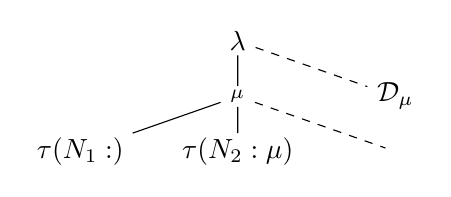
\begin{tikzpicture}[level distance=7mm,inner ysep=0.5mm,sibling distance=20mm]
\node {$\lambda$}
child[missing]{}
child {
    node {$\iaseq_\mu$}
    child{node{$\tau(N_1:\iacom)$}}
    child{node{$\tau(N_2:\mu)$}}
    child { node {\iadone} edge from parent[dashed] }
}
child{node{$\mathcal{D}_\mu$} edge from parent[dashed]};
\end{tikzpicture}
\\ \\
$\iamkvar\ N_w\ N_r :\iavar$ &
\begin{tikzpicture}
\matrix (m) [matrix of math nodes, row sep=5mm]
{
  \lambda^r & \lambda^{w_0} & \lambda^{w_1}  & \lambda^{w_2} & \lambda^{w_{\ldots}} \\
    \mathcal{D}_\iaexp &  & \iamkvar & & \iadone \\
    & \tau(N_r) & \tau(N_w) & \mathcal{D}_\iaexp & \iadone \\
};
\draw[-] (m-1-1) -- (m-2-3)
         (m-1-2) -- (m-2-3)
         (m-1-3) -- (m-2-3)
         (m-1-4) -- (m-2-3)
         (m-1-5) -- (m-2-3)
         (m-2-3) -- (m-3-2)
         (m-2-3) -- (m-3-3);
\draw[dashed] (m-2-3) -- (m-3-4)
              (m-2-3) -- (m-3-5)
              (m-1-1) -- (m-2-1)
              (m-1-5) -- (m-2-5)
              (m-1-4) -- (m-2-5)
              (m-1-3) -- (m-2-5)
              (m-1-2) -- (m-2-5);
\end{tikzpicture}
\\ \\
\parbox{3cm}{$\ianewin{x}\ N : \mu$ \\ $\mu \in \{ \iacom, \iaexp \} $} &
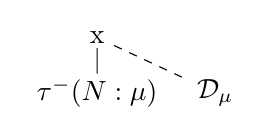
\begin{tikzpicture}[level distance=7mm,inner ysep=0.5mm,sibling distance=15mm]
\node {\ianewin{x}}
child[missing]{}
child{node{$\tau^-(N:\mu)$}}
child { node {$\mathcal{D}_\mu$} edge from parent[dashed]};
\end{tikzpicture}
\end{tabular}
\bigskip

where $\tau^-(N)$ denotes the DAG obtained by removing the root nodes from $\tau^-(N)$.
\end{center}
  \caption{Computation DAGs for the constructs of \ialgol.}
  \label{tab:ia_computationdag}
\end{table}


\subsubsection{Traversals}
Let $p$ be a node and suppose that its $i$th child $n$ has the
return type \iavar. Then $n$ is in fact constituted of several
$\lambda$-nodes : $\lambda^r \overline{\xi}$, $\lambda^{w_0}
\overline{\xi}$, \ldots. From $p$'s point of view, these nodes are
referenced as follows: $i.r$ refers to $\lambda^r \overline{\xi}$
and  $i.w_k$ refers to $\lambda^{w_k} \overline{\xi}$ for $k \in
\omega$.

\begin{itemize}
\item \emph{The application rule}

There are two rules (app$_{\iaexp}$) and (app$_{\iacom}$)
corresponding to traversals ending with an @-node of return type
\iaexp\ and \iacom\ respectively. These rules are identical to the
rule \iaexp\ of section \ref{subsec:traversal}.

The application rule for $@$-nodes with return type \iavar\ is:
$$(\mbox{app}_{\iavar})
\rulef{ \Pstr{t \cdot (lHyp){\lambda^k \overline{\xi}} \cdot
(appHyp-lHyp,35:0){@} \in \travset }
 }{\Pstr[18pt] {t \cdot (l){\lambda^k
\overline{\xi}} \cdot (app-l,35:0){@} \cdot (l2-app,35:0.k){\lambda^k
\overline{\eta}} \in \travset }}
 \ k \in \{ r, w_0, w_1, \ldots \}
$$


\item \emph{Input-variable rules}

There are two rules (InputVar$^{\iaexp}$) and (InputVar$^{\iacom}$)
which are the counterparts of rule (InputVar$^0$) of section
\ref{subsec:traversal} and are defined identically.

Let $x$ be an input-variable of type \iavar:
$$ (\mbox{InputVar}^{\iavar})
\rulef{t \cdot \lambda^r \overline{\xi} \cdot x \in \travset}
    {t \cdot \lambda^r \overline{\xi} \cdot \rnode{x}{x} \cdot v_x \in \travset }
\hspace{2cm} (\mbox{InputVar}^{' \iavar}) \rulef{t \cdot
\lambda^{w_i} \overline{\xi} \cdot x \in \travset}
    {t \cdot \lambda^{w_i} \overline{\xi} \cdot \rnode{x}{x} \cdot \iadone_x \in \travset }
$$

\item \emph{IA constants rules}

The rules for \ianew\ are purely structural, they are defined the
same way as the rules (app$_{\iaexp}$), (app$_{\iacom}$) and
(app$_{\iadone}$).

The rules for \iaderef\ are:
$$(\mbox{deref}) \rulef{t \cdot \iaderef \in \travset}{\Pstr[15pt]{t \cdot (d){\iaderef} \cdot (n-d,35:1.r){n} \in \travset }}
 \hspace{1.6cm} (\mbox{deref'})
\rulef{t \cdot \iaderef \cdot n \cdot t_2 \cdot v_n \in \travset} {t
\cdot \iaderef \cdot n \cdot t_2 \cdot v_n \cdot v_{\iaderef}\in
\travset }
$$


The rules for \iaassign\ are:
$$(\mbox{assign}) \rulef{t \cdot \iaassign \in \travset}{\Pstr[15pt]{t \cdot (ass){\iaassign} \cdot (n-ass,35:1){n} \in \travset} }
\hspace{1.6cm}
(\mbox{assign'})
\rulef{t \cdot \iaassign \cdot n \cdot t_2 \cdot v_n \in
\travset} {\Pstr[18pt]{t \cdot (ass){\iaassign} \cdot (n){n} \cdot
t_2 \cdot v_n \cdot (m-ass,15:2.w_n){m} \in \travset } }
$$
$$(\mbox{assign''})  \rulef{\Pstr{t \cdot (assHyp){\iaassign} \cdot t_2 \cdot (mHyp-assHyp,35:2.w_k){m} \cdot t_3 \cdot \iadone_m \in \travset}}
{t \cdot \iaassign \cdot t_2 \cdot m \cdot t_3 \cdot \iadone_m \cdot
\iadone_{\iaassign} \in \travset }
$$

The rules for $\iaseq_{\iaexp}$ are:
$$(\mbox{seq}) \rulef{t \cdot \iaseq \in \travset}{\Pstr[13pt]{t \cdot (seq){\iaseq} \cdot (n-seq,35:1){n} \in \travset } }
\hspace{1.6cm} (\mbox{seq'})
\rulef{t \cdot \iaseq \cdot n \cdot t_2 \cdot v_n \in
\travset} {\Pstr[18pt]{ t \cdot (seq){\iaseq} \cdot (n){n} \cdot t_2
\cdot v_n \cdot (m-seq,25:2){m} \in \travset }}
$$
$$(\mbox{seq''})  \rulef{\Pstr{t \cdot (seqHyp){\iaseq} \cdot t_2 \cdot (mHyp-seqHyp,35:2){m} \cdot t_3 \cdot v_m \in \travset}}
{t \cdot \iaseq \cdot t_2 \cdot m \cdot t_3 \cdot v_m \cdot
v_{\iaseq} \in \travset }$$




The rules for \iamkvar\ are:
$$(\mbox{mkvar}_r) \rulef{t \cdot \lambda^r \overline{\xi} \cdot \iamkvar \in \travset}{\Pstr[14pt]{t \cdot \lambda^r \overline{\xi} \cdot (d){\iamkvar} \cdot (n-d,35:1){n} \in \travset} }
\hspace{1cm} (\mbox{mkvar}_r')
\rulef{t \cdot \iamkvar \cdot n \cdot t_2 \cdot v_n \in \travset} {t
\cdot \iamkvar \cdot n \cdot t_2 \cdot v_n \cdot v_{\iamkvar}\in
\travset } $$
$$(\mbox{mkvar}_w) \rulef{t \cdot \lambda^{w_k} \overline{\xi} \cdot \iamkvar \in \travset}{\Pstr[15pt]{t \cdot \lambda^{w_k} \overline{\xi} \cdot (mk){\iamkvar} \cdot (n-mk,35:2){n} \in \travset} }$$
$$ (\mbox{mkvar}_w'')  \rulef{t \cdot \lambda^{w_k} \overline{\xi} \cdot \iamkvar \cdot n \cdot t_2 \cdot \iadone_n \in \travset}
{t \cdot \lambda^{w_k} \overline{\xi} \cdot \iamkvar \cdot n \cdot
t_2 \cdot \iadone_n \cdot \iadone_{\iamkvar} \in \travset }
$$
These four rules are not sufficient to model the constant \iamkvar.
Indeed, consider the term $\iaassign\ (\iamkvar\ (\lambda x . M) N)
7$. The rule (\mbox{mkvar}$_w''$) permits to traverse the node
\iamkvar\ and to go on by traversing the computation tree of
$\lambda x . M$. The problem is that when traversing $\tau(M)$, if
we reach a variable $x$, we are not able to relate $x$ to the value
$7$ that is assigned to the variable.

To overcome this problem, we need to define traversal rules for
variable in such a way that a variable node bound by the second
child of a $\iamkvar$-node is treated differently from other
variables.

\item \emph{Variable rules}
Let $x$ be a non input-variable node. It either corresponds to a $\lambda$-abstracted variable or
a block-allocated variable declared by the $\ianewin{x}$ construct.

\begin{itemize}
\item Suppose that $x$ is $\lambda$-abstracted and let $\lambda \overline{x}$ be its binder.
In \ialgol, the only constant nodes of order greater than 1 is
\iamkvar, therefore there are two cases: $\lambda \overline{x}$ is
either the child of a node in $N_@ \union N_{\sf var}$ or it is the
second child of a \iamkvar-node.

To handle the first case, we define a rule similar to the (Var) rule
of section \ref{subsec:traversal} with some modification to take
into account variables $x$ of type \iavar (in which case $x$ has
multiple parent $\lambda$-nodes). We do not give the details here
but it is easy to see how to redefine this rule.

To handle the case where $\lambda \overline{x}$ is the child of a
\iamkvar-node, we define the following rule:
$$ (\mbox{Var}_{\iamkvar})  \rulef{t \cdot \lambda^{w_k} \overline{\xi} \cdot \iamkvar \cdot \lambda \overline{x} \cdot t_2 \cdot x \in \travset}
{t \cdot \lambda^{w_k} \overline{\xi} \cdot \iamkvar \cdot \lambda
\overline{x} \cdot t_2 \cdot x \cdot k_{x} \in \travset }
$$

\item Suppose that $x$ is block-allocated with $\ianewin{x}$.

We call \emph{overwrite of $x$ relatively to an occurrence of a} ``\ianewin{x}''\emph{-node}, any sequence of nodes of the form
$\Pstr[17pt]{(decl){\ianewin{x}}\cdot \ldots \cdot \lambda^{w_k}\overline{\xi} \cdot (x-decl,25){x}}$ for some $k\in \mathcal{D}_{\iaexp}$ and node $\lambda^{w_k}\overline{\xi}$ parent
of $x$.
$$(\mbox{Var}_w)
    \rulef{
        t \cdot \lambda^{w_k} \overline{\xi} \cdot x \in \travset
    }
    {   t \cdot \lambda^{w_k} \overline{\xi} \cdot x \cdot \iadone_x \in
        \travset
    },
$$

$$(\mbox{Var}_r)
    \rulef{
        \Pstr[17pt]{t_1 \cdot (decl){\ianewin{x}} \cdot t_2 \cdot \lambda^r \overline{\xi} \cdot (x-decl,25){x} \in \travset}
    }
    {   t_1 \cdot \ianewin{x} \cdot t_2 \cdot \lambda^r \overline{\xi}
        \cdot x \cdot 0_x \in \travset
    }
    \mbox{ if $t_2$ contains no overwrite of $x$},
$$

$$(\mbox{Var'}_r)
    \rulef{
        \Pstr[15pt]{
            t_1 \cdot (decl){\ianewin{x}} \cdot t_2 \cdot \lambda^r \overline{\xi} \cdot (x-decl,25){x} \in \travset
        }
    }
    {
        t_1 \cdot \ianewin{x} \cdot t_2 \cdot \lambda^r \overline{\xi} \cdot x \cdot k_x \in \travset
    }
    \mbox{ if $\lambda^{w_k} \cdot x$ is the last overwrite of $x$ in } t_2. $$
\end{itemize}
\end{itemize}

\subsubsection{Game semantics correspondence}
The properties that we proved for computation trees and traversals
of the safe $\lambda$-calculus with constants can easily be lifted
to computation DAGs of \ialgol. In particular:
\begin{itemize}
\item constant traversal rules are well-behaved (for order-$0$ and order-$1$ constants, this is a consequence
of Lemma \ref{lem:sigma_order1_are_wellbehaved}; for $\iamkvar$
however it needs to be proved separately);
\item P-view of traversals are paths in the computation DAG;
\item the P-view of the reduction of a traversal is the reduction of the P-view,
and the O-view of a traversal is the O-view of its reduction
(Lemma \ref{lem:pview_trav_projection} and
\ref{lem:oview_trav_projection});
\item there is a mapping from vertices of the computation DAG to moves in the interaction game semantics;
\item there is a correspondence between traversals of the computation tree and plays in interaction game semantics;
\item consequently, there is a correspondence between the standard game semantics and
the set of justified sequences of nodes $\travset(M)^{\filter
\theroot}$.
\end{itemize}

\subsubsection{Game-semantic characterisation of safe terms}
Clearly, the computation DAG of a safe term is incrementally-bound.
By using the correspondence between traversals and plays, it is easy
to prove that incrementally-bound computation trees are denoted by
P-incrementally-justified strategies. Consequently, by lemma
\ref{lem:incrjustified_pointers_uniqu_recover}, P's pointers are superfluous in the
game semantics of safe \ialgol\ terms.

Since the game denotation of an \ialgol\ term is fully determined by
the set of complete plays, this pointer economy suggests that the
game denotation of a safe \ialgol\ can be represented in a compact
way. This raises the question of the decidability of observational
equivalence for safe \ialgol.



%%%%%%%%%%%%%%%%%%%%%%%%%%%%
%%%%%%%%%%%%%%%%%%%%%%%%%%%%
\notetoself{the following section needs to be integrate into the previous chapter.}


\section{Game-semantic of Safe PCF}
In this section will give a game-semantic characterization of Safe
PCF based on syntactical arguments.

\begin{definition}
We say that a PCF term is \defname{semi-safe} if it is of the form
$N_0 N_1 \ldots N_k$ for $k\geq 1$ where each of the $N_i$ is a Safe
PCF term or if it can be written $\lambda \overline{x} . N$ for some
safe PCF term $N$.
\end{definition}
Semi-safe terms are either safe or ``almost safe'' in the sense that
they can be turned into an equivalent (i.e.~with isomorphic game
semantics) safe term  by performing $\eta$-expansions. Indeed, let
$M$ be an semi-safe term that is unsafe. If $M$ is of the first form
$N_0 N_1 \ldots N_k : (A_1,\ldots,A_n)$ with $k\geq 1$ then let
$\varphi_i:A_i$ for $i\in\{1..n\}$ be fresh variables, using the
(app) and (abs) rules we can build the safe term $\lambda \varphi_1
\ldots \varphi_n . N_0 N_1 \ldots N_k \varphi_1 \ldots \varphi_n$.
If $M$ is of the second form $\lambda \overline{x} . N$ then using
the abstraction rule we can build the equivalent safe term $\lambda
\overline{y} \overline{x}. N$  where $\overline{y} = fv(\lambda
\overline{x}. N)$.

The $\beta$-normal form of a \pcf\ term is the possibly infinite
term obtained by reducing all the redexes in $M$.

\subsubsection{Safe terms vs P-i.j.\ strategies}

In the context of the simply typed lambda calculus, the
correspondence between safety and P-incremental justification was
first shown in \cite[Theorem 3(ii)]{blumong:safelambdacalculus}
using a syntactic argument:
\begin{theorem}[\cite{blumong:safelambdacalculus},Theorem 3(ii)]
\label{thm:safeincrejust}
 In the simply typed lambda calculus:
\begin{enumerate}[(i)]
\item If $M$ is safe then $\sem{M}$ is P-incrementally justified.
\item If $M$ is a closed term and $\sem{M}$ is
  P-incrementally justified then the $\eta$-long form of the
  $\beta$-normal form of $M$ is safe.
\end{enumerate}
\end{theorem}
In fact the following more precise result holds (the proof of the
previous theorem can be easily adapted to this one):
\begin{theorem}[Semi-safety and P-incremental justification]
\label{thm:semisafeincrejust} Let $\Gamma \vdash M : A$ be a simply typed term. Then:
\begin{enumerate}[(i)]
\item If $\Gamma \vdash M : A$ is semi-safe then $\sem{\Gamma \vdash M : A}$ is P-incrementally justified.
\item If $\sem{\Gamma \vdash M : A}$ is
  P-incrementally justified then $\etalnf{\betanf{M}}$ is
semi-safe if $M$ is open and safe if $M$ is closed.
\end{enumerate}
\end{theorem}



In the context of \pcf\ however, only the first part of the theorem
holds (see \cite{blumtransfer} for the proof). However (ii) does not
hold. Indeed, take the closed \pcf\ term $M = \lambda f x y. f
(\lambda z. \pcfcond (\pcfsucc\ x) y z )$ where $x,y,z:o$ and
$f:((o,o),o)$. $M$ is in normal form (conditional cannot be reduced
since the value of $x$ is undetermined). The $\eta$-long form of the
$\beta$-normal form of $M$ is therefore $M$ itself which is unsafe.
But clearly we have $\sem{M} = \sem{\lambda f x y. f (\lambda z.
z)}$, and since $\lambda f x y. f (\lambda z. z)$ is safe, by (i),
$\sem{M}$ is P-incrementally justified.

Such counter-example arises because the conditional operator of
\pcf\ permits us to construct terms in normal form that contain
``dead code'' {\it i.e.}~some subterm that will never be evaluated
for any value of M's parameters. In the example above, the dead code
consists of the subterm $y$. In general, if the dead code part of
the computation tree contains a variable that is not incrementally
bound then the resulting term will be unsafe even if the rest of the
tree is incrementally bound. In the example above, it was possible
to turn $M$ into the equivalent safe term $\lambda f x y. f (\lambda
z. z)$ by eliminating the dead code from $M$. In fact we can
generalise this method to any \pcf\ term with a P-incrementally
justified denotation.
\smallskip

Dead code elimination can be difficult to achieve in practice but it
is easy to define it formally: We say that a subterm $N$ occurring
in a context $C[-]$ in $M : (A_1, \ldots, A_n,o)$ is part of the
\defname{dead code} of $M$ if for any term $T_0$ of the form $M M_1
\ldots M_n$, any reduction sequence starting from $T_0$ does not
involve a reduction of the subterm $N$ {\it i.e.}~for any reduction
sequence $T_0 \redar T_1 \redar \ldots \redar T_k$, there is no
$j\in \{0.. k-1\}$ such that $T_j = C[N]$ and $T_{j+1} = C[N']$ for
some term $N'$.


Let $M$  be a \pcf\ term in $\eta$-nf. An occurrence of a variable
$x$ in $M$ is said to be a \defname{dead occurrence} if it occurs in
the dead code of $M$. In other words, it is a dead occurrence of $x$
if the corresponding node in the computation tree does not appear in
any traversal of $\travset(M)$. Equivalently, thanks to the
Correspondence Theorem, an occurrence of $x:B$ is dead if and only
if the initial move of the arena $\sem{B}$ does not appear in any
play of $\sem{M}$.


We define $M^*$ as the term obtained from $M$ after substituting all
subterms of the form  $x N_1 \dots N_k$ for some dead variable
occurrence $x:(B_1,\ldots, B_k, o)$ by the constant $0$. This
process is called \defname{dead variable elimination}. Note that if
$M$ is in $\eta\beta$-nf then so is $M^*$. We also write $\tau(M)^*$
to denote the equivalent transformation on the computation tree.
Since the computation tree is constructed from the $\eta$-nf of $M$,
we will use this notation even when $M$ is not in $\eta$-nf.



\begin{proposition}[Incremental-binding and P-incremental justification coincide] \
\label{prop:Nher_incrbound_and_incrjustified_pcf} Let $\Gamma \vdash
M : A$ be a PCF term in $\beta$-normal form.
\begin{enumerate}[(i)]
\item  If $\tau(\Gamma \vdash M : A)$ is incrementally-bound then $\sem{\Gamma \vdash M : A}$ is P-incrementally justified,
\item  if $\sem{\Gamma \vdash M : A}$ is P-incrementally justified
then $\tau(\Gamma \vdash M : A)^*$ is incrementally-bound.
\end{enumerate}
\end{proposition}
\begin{proof}
(i) The proof is exactly the same as in the simply typed lambda calculus case,
see \cite[Proposition 4.1.5(i)]{blumtransfer}.

\noindent (ii)
Take $\Gamma \vdash M : A$ a \pcf\ term in $\beta$-normal form denoted by $\sem{\Gamma \vdash M : A}$ P-incrementally justified. Let $r$ denote the root of $\tau(M)^*$.
Let $n$ be a node of $\tau(M)^*$ labelled by the variable $x$.
$\tau(M)^*$ is free from dead code therefore $n$ is not a dead occurrence of $x$ and there exists a traversal of $\tau(M)^*$ of the form $t \cdot x$.

\pcf\ constants are of order $1$ at most therefore they cannot
hereditarily justify a variable node, thus $x$ is necessarily
hereditarily justified by the only occurrence $r$ of the root of the
computation tree.

By considering $t\cdot x$ as a traversal of $\tau(M)$,  the
correspondence theorem gives $\varphi((t \cdot x) \filter r) =
\varphi((t \filter r) \cdot x) \in \sem{M}$. Since $\sem{M}$ is
P-incrementally justified, $\varphi(x)$ must point to the last
O-move in $\pview{\varphi(t \filter r)}$ with order strictly greater
than $\ord{\varphi(x)}$. Consequently $x$ points to the last node in
$\pview{t \filter r} \filter N^{\lambda}$ with order strictly
greater than $\ord{x}$. We have:
\begin{align*}
\pview{t \filter r} &= \pview{t} \filter N^{r \vdash} & (\mbox{by Lemma \ref{lem:betanf_wellbehavedconst_trav_pview_red}}) \\
& = [r,x[ \ \filter N^{r \vdash} & (\mbox{by Prop.\ \ref{prop:pviewtrav_is_path}})
\end{align*}
\notetoself{review use of Lemma
\ref{lem:betanf_wellbehavedconst_trav_pview_red}}

Since $M$ is in $\beta$-nf, the set of nodes not hereditarily
enabled by $r$ is exactly the set of nodes hereditarily enabled by
$N_{\Sigma}$ thus $[r,x[ \ \filter N^{r \vdash} = [r,x[\ \setminus\
N^{\filter \Sigma}$. Moreover \pcf\ constants are of order $1$ at
most therefore $N^{\filter \Sigma} = N_{\Sigma} \union N^c_{\Sigma}$
where $N^c_{\Sigma}$ is the set of children nodes of $N_{\Sigma}$.
Thus $\pview{t \filter r} \filter N^{\lambda} = ([r,x[\ \setminus\
N_{\Sigma} \setminus N^c_{\Sigma} ) \filter N^{\lambda} = ([r,x[\
\setminus\  N^c_{\Sigma} )  \filter N^{\lambda}$, and since
$N^c_{\Sigma}$ is constituted of order $0$ lambda-nodes only, $x$
must point to the last node in $[r,x[ \filter N^{\lambda}$ with
order strictly greater than $\ord{x}$.

Hence if $x$ is a bound variable node then it is bound by the
last $\lambda$-node in $[r,x[$ with order strictly greater than
$\ord{x}$ and if $x$ is a free variable then it points to $r$ and
therefore all the $\lambda$-node in $]r,x[$ have order smaller than
$\ord{x}$. Thus $\tau(M)^*$ is incrementally-bound.
\end{proof}

The counterpart of Lemma 4.1.6 from
\cite{blumtransfer} can be stated as follows in the context of PCF:
\begin{lemma}[Semi-safety and incrementally-binding]
\label{lem:incrbound_iff_etanf_safe_pcf} Let $\Gamma \vdash M : A$
be a PCF term.
\begin{itemize}
\item[(i)] If $\Gamma \vdash M : A$ is a semi-safe term then $\tau(\Gamma \vdash M : A)$ is incrementally-bound ;
\item[(ii)] conversely, if $\tau(\Gamma \vdash M : A)$ is incrementally-bound then the $\eta$-normal form of $\Gamma \vdash M : A$ is semi-safe if $M$ is open and safe if $M$ is closed.
\end{itemize}
\end{lemma}
The proof can be obtained by adapting the proof
of Lemma 4.1.6 from \cite{blumtransfer}.

\begin{theorem}[Semi-safety and P-incremental justification]
\label{thm:semisafeincrejust_pcf} Let $\Gamma \vdash M : A$ be a PCF term. Then:
\begin{enumerate}[(i)]
\item If $\Gamma \vdash M : A$ is semi-safe then $\sem{\Gamma \vdash M : A}$ is P-incrementally justified.
\item If $\sem{\Gamma \vdash M : A}$ is
  P-incrementally justified then $\etalnf{\betanf{M}}^*$ is
  semi-safe  if $M$ is open, and safe if $M$ is closed.
\end{enumerate}
\end{theorem}

\begin{proof}
\noindent(i)
A proof of this is given in the proof of Theorem 4.2.10 in \cite{blumtransfer}.

\noindent(ii) Suppose $M$ is a \pcf\ term with a P-incrementally
justified strategy denotation. By Proposition
\ref{prop:Nher_incrbound_and_incrjustified_pcf}(ii),
$\tau(\betanf{M})^* = \tau(\etalnf{\betanf{M}}^*)$ is
incrementally-bound. If $M$ is closed then so is
$\etalnf{\betanf{M}}^*$ therefore by Lemma
\ref{lem:incrbound_iff_etanf_safe_pcf},
$\etalnf{\etalnf{\betanf{M}}^*} = \etalnf{\betanf{M}}^*$ is safe. If
$M$ is open then so is $\etalnf{\betanf{M}}^*$ and by Lemma
\ref{lem:incrbound_iff_etanf_safe_pcf},
$\etalnf{\etalnf{\betanf{M}}^*} = \etalnf{\betanf{M}}^*$ is
semi-safe.
\end{proof}


We write \pcf' to denote the language obtained by extending \pcf\
with the $\pcfcase_k$ construct (see \cite{Abr02}).
The $\pcfcase_k$ construct is the obvious generalisation of the
conditional operator \pcfcond\ to $k$ branches instead of $2$. All the results obtained so far concerning Safe \pcf\ (including those
cited from \cite{blumtransfer}) can clearly be transposed to \pcf'.

\subsubsection{Definability result}

The previous theorem leads to the following definability result for safe \pcf':
\begin{proposition}[Definability for safe \pcf' terms]
\label{prop:safetydefinability} Let $\overline{A}=(A_1,\ldots, A_i)$
and $B =(B_1, \ldots, B_l,o)$ be two PCF types for some $i,l\geq 0$
and $\sigma$ be a well-bracketed innocent P-i.j.\ strategy with
finite view function defined on the game $!A_1 \otimes \ldots
\otimes !A_i \lingamear (!B_1 \lingamear \ldots \lingamear !B_l
\lingamear o) $. There exists a \emph{semi-safe} PCF' term
$\overline{x} : \overline{A} \vdash M : B$ in $\eta$-long normal
form such that:
$$ \sem{\overline{x} : \overline{A} \vdash M_\sigma : B} = \sigma $$
and a safe closed PCF' term $\vdash_s M'_\sigma : (\overline{A},B)$ in $\eta$-long normal form such that:
$$ \sem{\vdash M'_\sigma : (\overline{A},B)} \cong \sigma \ .$$
\end{proposition}
\begin{proof}
By the standard definability result for PCF', there is a term
$\overline{x} : \overline{A} \vdash N : B$ such that
$\sem{\overline{x} :\overline{A} \vdash N : B} = \sigma$. Take
$M_\sigma$ to be $\etalnf{\betanf{N}}^* $. We have
$\sem{\overline{x} : \overline{A} \vdash M_\sigma : B} =
\sem{\overline{x} :\overline{A} \vdash N : B} = \sigma$ and by
Theorem  \ref{thm:semisafeincrejust_pcf}(ii), $M_\sigma$ is
semi-safe. For the second part we just need to take $M'_\sigma =
\lambda \overline{x}. M_\sigma$.
\end{proof}



\subsubsection{Compositionality of P-i.j.\ strategies (syntactic
argument)}


We have already shown in Sec. \ref{sec:closedpij} that under certain
conditions, P-i.j.\ strategies compose. Here we will obtain a
slightly weaker version of this result using a much simpler argument
which exploits the definability result from the previous section.


 Let $\overline{A} = (A_1, \ldots, A_i)$, $B = (B_1, \ldots,
B_l,o)$ and $C=(C_1,\ldots,C_k,o)$ be three PCF types for some
$i\geq 1,l,k\geq 0$. Let $f:\ !A_1 \otimes \ldots \otimes !A_i
\lingamear B$ and $g:\ !B\lingamear C$ be two innocent
well-bracketed and P-incrementally justified strategies with finite
view function. We would like to find under which conditions the
composition $f\fatcompos g$ is also P-incrementally justified.

By the definability result, there are two closed safe terms (in $\eta$-nf) $\vdash M_f :(\overline{A},B)$  and $\vdash M_g :B \typear C$ such that $\sem{M_f} = f$
and $\sem{M_f} = g$.
We define the term $M_{f\fatcompos g} = \lambda \overline{x} . M_g (M_f \overline{x})$ for some fresh variables $\overline{x} : \overline{A}$. Clearly we have $\sem{M_{f\fatcompos g}} = \sem{M_f} \fatcompos \sem{M_g} = f\fatcompos g$.

\paragraph{Sufficient conditions}

By Theorem \ref{thm:semisafeincrejust_pcf}, we know that
$f\fatcompos g$ is P-incrementally justified just when
$\etalnf{\betanf{M_{f\fatcompos g}}}^*$ is safe. We will now exploit
this fact to extract a sufficient condition on the types $A$ and $B$
for the composition of $f$ and $g$ to be P-incrementally justified.

The term $M_f$ and $M_g$, being in $\eta$-nf, are of the following forms:
\begin{eqnarray*}
\vdash M_f &=& \lambda x_1^{A_1} \ldots x_i^{A_i} \varphi_1^{B_1} \ldots \varphi_l^{B_l} . N_f^o\\
\vdash  M_g &=& \lambda y^{ (B_1, \ldots, B_l,o)} \phi_1^{C_1} \ldots \phi_k^{C_k} . N_g^o
\end{eqnarray*}
for some distinct variables $x_1, \ldots, x_i$, $y$, $\varphi_1, \dots \varphi_l$, $\phi_1, \dots \phi_k$  and $\eta$-normal terms $N_f$ and $N_g$:
\begin{eqnarray*}
x_1:A, \ldots, x_i:A_i, \varphi_1:B_1, \dots, \varphi_l:B_l &\vdash& N_f :o \\
y: (B_1, \ldots, B_l,o), \phi_1:C_1, \dots, \phi_l:C_l &\vdash& N_g :o
\end{eqnarray*}



The fact that $M_f$ and $M_g$ are safe does not imply that $M_{f\fatcompos g}$ is: take $M_f = \lambda x^o z^o.x$ and $M_g = \lambda y^{(o,o)} . y a$ for some constant $a\in \Sigma$, then $\lambda x:A . M_g (M_f x) = \lambda x . (\lambda y . y a) ( \underline{(\lambda x z.x) x} )$ is unsafe because of the underlined subterm. However we have:
\begin{align*}
f\fatcompos g &= \sem{\lambda \overline{x} . M_g (M_f  \overline{x})} \\
 &= \sem{\lambda \overline{x} . (\lambda \phi_1\ldots \phi_k . N_g) [(M_f \overline{x}) / y]} \\
&= \sem{\lambda \overline{x} \phi_1 \dots \phi_k. N_g [(M_f  \overline{x}) / y]}
& \mbox{(the $x_j$'s and $\phi_j$'s are disjoint)}.
\end{align*}

We now concentrate on the term  $\lambda \overline{x} \phi_1 \dots
\phi_k. N_g [(M_f  \overline{x}) / y]$ and try to find a sufficient
condition guaranteeing its safety.

\subparagraph{A sufficient condition}
\begin{lemma}
Suppose that $\Gamma,y:B \vdash M$ is a safe term in $\eta$-nf and $\Gamma \vdash R : B$ is an almost safe application. Let $N$ denote the set of nodes of the computation tree $\tau(M)$. We have:
\begin{align*}
\Gamma \vdash M[R/y] :A \mbox{ safe }
\iff&  \forall x \in fv(R) . \\
    & \forall n_y \in N_{\sf fv} \mbox{ labelled $y$}.
      \forall m \in N_{\lambda} \inter ]r,n_y] : \ord{m} \leq \ord{x}
\end{align*}
\end{lemma}
\begin{proof}
Since $M$ is in $\eta$-nf, all the application to the variable $y$ are total (i.e.~of the form $y P_1 \ldots P_l :o$). Hence after substituting the safe term $N$ for $y$ in $M$, the only possible cause of unsafety is when
some variable free in $N$ becomes not safely bound in $\tau(M)$.
\end{proof}

Applying this lemma with $R= M_f \overline{x}$ gives us a sufficient
condition -- the right-hand side of the equivalence -- for $\lambda
x \phi_1 \dots \phi_k. N_g [(M_f \overline{x}) / y]$ to be safe, and
hence for $f\fatcompos g$ to be P-incrementally justified. Of course
it is not a necessary condition since $N_g[(M_f \overline{x}) /y]$
can be unsafe while its eta-beta normal form is safe.

\subparagraph{A simpler sufficient condition}
\begin{lemma}
If $y:B, \Sigma \vdash N : T$ and $\vdash M : (\overline{A}, B)$
are safe terms with $\ord{A_i} \geq \ord{B}$ for all $i\in 1..n$
then $\overline{x}:\overline{A}, \Sigma \vdash N[(M \overline{x})/y] :T$ is also safe.
\end{lemma}
\begin{proof}
Since $\ord{x_i} = \ord{A_i} \geq \ord{B} = \ord{M \overline{x}}$, we can use the application
rule of the safe lambda calculus to form the safe term $\overline{x}:\overline{A} \vdash M \overline{x}$.
Using the substitution lemma we have that $N[(M \overline{x})/y]$ is safe.
\end{proof}

Hence we obtain the following sufficient condition for $f\fatcompos
g$ to be P-incrementally justified:
$$\ord{A_i}\geq\ord{B} \mbox{ for all } 1 \leq i \leq n$$


Indeed the lemma gives that $\vdash \lambda \overline{x} \phi_1
\dots \phi_k. N_g [(M_f \overline{x}) / y]$ is safe and therefore
its denotation $\sem{\vdash \lambda \overline{x} \phi_1 \dots
\phi_k. N_g [(M_f \overline{x}) / y]} = f\fatcompos g$ is
P-incrementally justified.

Note that this condition is not necessary: Take $A=o$, $B=(o,o)$,
$C=(o,o)$ and consider the two safe terms $M_f = \lambda x^A u^o.u$
and $M_g = \lambda y^B . y a$ for  some constant $a:o$. Then we have
$M_{f\fatcompos g} = \lambda x . a$ which is safe hence $f\fatcompos
g$ is P-incrementally justified although $\ord{A} < \ord{B}$.

\begin{remark}
This result corroborates what we already know about compositionality
of P-i.j.\ strategies (see Sec. \ref{sec:closedpij}). Indeed, the
condition given hereinbefore implies that the strategy $f$ is
\emph{closed} P-i.j.\ (the $A_i$s are prime because we are working
with PCF types) and therefore by Prop.\ \ref{prop:closedpijcompose},
$f \fatcompos g$ must also be P-i.j.
\end{remark}




\paragraph{Counter-example: two P-i.j.\ strategies whose composition is not
P-i.j.}

We now give counter-example to show that P-i.j.\ strategies do not
compose in general.

\subparagraph{First attempt}

Take the types $A=o$, $B=(o,o)$, $C=o$, the variables
$x,u,v:o$, $y:B$ and $\varphi:((o,o),o)$ and $\Sigma$-constant $a:o$.
Consider the two safe terms $\vdash_s  M_f = \lambda xv.x : A\typear B$ and $\vdash_s M_g = \lambda y . \varphi (\lambda u . y a) : B\typear C$.
The $\eta\beta$-nf of $M_{f\fatcompos g}$ is $\vdash \lambda x . \varphi (\underline{\lambda u . x})$ which is unsafe because of the underlined term. It is then tempting to use
Theorem \ref{thm:safeincrejust}(ii) to conclude that
$\sem{M_{f\fatcompos g}}$ is not P-incrementally justified. However this theorem cannot be used here because $M_g$ contains an order $2$ constants ($\varphi$) therefore
$M_{f\fatcompos g}$ is not a valid simply typed $\lambda$-term (nor a \pcf-term).

\subparagraph{Second attempt} The previous example can be easily
changed into a working counter-example: we just need to elevate
$\varphi$ from the status of constant to variable.

Take $A=o$, $B=(o,o)$, $C=(((o,o),o),o)$, the variables
$x,u,v:o$, $y:B$ and $\varphi:((o,o),o)$ and the $\Sigma$-constant $a:o$. Consider the two safe terms $\vdash_s  M_f = \lambda xv.x : A\typear B$ and  $\vdash_s M_g = \lambda y \varphi. \varphi (\lambda u . y a) : B\typear C$.
The $\eta\beta$-nf of $M_{f\fatcompos g}$ is $\vdash \lambda x \varphi. \varphi (\underline{\lambda u . x})$ which is unsafe because of the underlined term, thus by Theorem \ref{thm:safeincrejust}(ii), $\sem{M_{f\fatcompos g}}=\sem{M_f} \fatcompos
\sem{M_g}$ is not P-incrementally justified. The following diagram illustrates a play that is not P-i.j.:

\begin{center}
\begin{tikzpicture}[style={anchor=base}]
\matrix (m) [matrix of math nodes]
{
    \ &   & \ & \ & \ & \ &  & &\  &  & & & \\
    o & \stackrel{\sigcol{\sem{M_f}}}\longrightarrow & (o, & o) & \stackrel{\mucol{\sem{M_g}}}\longrightarrow & (((o, &o),& o),& o) \\ \\
    &&&&&&&&\node(n0){\lambda x \varphi \omove  \mucol {\lambda y \varphi}};\\[3mm]
    &&&&&&&\node(n1){\varphi  \pmove \mucol \varphi};\\[3mm]
    &&&&&&\node(n2){\lambda u \omove  \mucol {\lambda u}}; \\[3mm]
    &&&  \node(n3){ \sigcol {\lambda x v} \opmove \mucol y}; \\[3mm]
    \node(n4){x \pmove \sigcol x}; \\
};
\draw [-,thick] (m-1-1.south west) -- (m-1-1.south east) node [above,midway] {A};
\draw [-,thick] (m-1-3.south west) -- (m-1-4.south east) node [above,midway] {B};
\draw [-,thick] (m-1-6.south west) -- (m-1-9.south east) node [above,midway] {C};
\path (n4) edge[tableptr] (n0);
\path (n2) edge[tableptr,\mucolor] (n1);
\path (n1) edge[tableptr,\mucolor] (n0);
\path (n3) edge[tableptr,\mucolor] (n0);
\path (n4) edge[tableptr,\sigcolor] (n3);
\end{tikzpicture}
\end{center}


\subparagraph{Another counter-example with $\ord{B} = \ord{C}$.}

Let $A=o$, $B=C=(((o,o),o),o)$ and let $x:A$, $y:B$, $u:o$, $v,\varphi:((o,o),o)$
and $g:(o,o)$ be variables and  $a:o$ be a $\Sigma$-constant. Take the two safe terms $\vdash  M_f = \lambda x v.x$ and $\vdash M_g = \lambda y \varphi. \varphi (\lambda u . y (\lambda g. a))$.
The $\eta\beta$-nf of $M_{f\fatcompos g}$ is $\vdash \lambda x \varphi. \varphi (\underline{\lambda u . x})$ which is unsafe because of the underlined term, so
$f\fatcompos g$ is not P-incrementally justified.
